\chapter{Social groups at Selwyn Girls' High}
\label{ch:ethnography}
\date{}





\section{Methodology}

\subsection{Background}

I was raised in Southern California, an ocean apart from the students of Selwyn Girls' High. Prior to joining them, my education experience in New Zealand was limited to the university and despite talking to several New Zealanders about what it had been like when they went to \isi{high school}, I still did not have a clear idea of what to expect. In her ethnography on New Zealand teenagers, \citet{gray1988} focused on what was important to adolescents (e.g., friends and family) and not on the construction of their \isi{social groups} or their \isi{identity}. I was unsure of how to proceed and uncertain about what I might find. I knew most students at most schools wore uniforms. I knew that I might not find an equivalent of the Jocks and Burnouts observed by \citet{eckert1989} and I entered the school thinking it possible that I may not find any distinct groups at all.\footnote{One colleague from New Zealand suggested that I might observe a hierarchy of ``coolness'' as opposed to distinct groups of students.}   


Selwyn Girls' High seemed the ideal school to conduct my analysis: It was an all girls' school with students from a range of socioeconomic backgrounds. I wanted to work in an all girls' school to observe adolescents' construction of \isi{identity} in the absence of members of the opposite sex. Previous work has focused on \isi{identity} construction within the context of the heterosexual marketplace \citep{eckert1996nailpolish}. Though the marketplace certainly still comes into play with girls from an all girls' school, they do not necessarily construct their school identities in the same way that girls at co-ed schools do. 

Schools in New Zealand are assigned a decile depending on how many of its students come from low socio-economic communities. Decile 1 schools are the 10\% of schools in New Zealand with the highest proportion of students from low socio-economic communites and decile 10 schools are the 10\% with the lowest proportion of students from low socio-economic communities.\footnote{Deciles are assigned so that schools with a high percentage of students from low socio-economic communities can receive more government funding.} At the time of the study, SGH had a decile of 6, which reflects the range of socio-economic backgrounds among its 1200 students. SGH was a public school and students came from very distinct parts of the city as well as from surrounding rural areas. This mixture of students from different backgrounds appealed to me. Given the ubiquity of class-based sociophonetic findings (e.g., \citet{labov1966}, \citet{trudgill1972}, observing an absence of socially-meaningful linguistic variation in this context would be surprising and given the aims of the project, observing variation that was socially-meaningful could be enlightening. Therefore, I felt confident that I would have some sociolinguistically interesting finding, whatever the outcome. \nocite{labov1966} \nocite{trudgill1972}

%I hypothesised that girls who were from different socioeconomic backgrounds from their friends might display phonetic variation that more closely reflects their friends' productions than the socioeconomic group to which they and their parents belong. 

\subsection{The students}
I focused on the girls in their 13th and final year of school. In New Zealand, \isi{high school} runs from Year 9 to Year 13.\footnote{In the past, `years' were referred to as `forms', where 7th form was the equivalent of Year 13.}  Most Year 13 students turn 18 during the course of the year. 

High school in New Zealand is not compulsory for students over 16. Though it is discouraged by teachers and many parents, students can choose to ``sign out'' of school and it does not have the same social stigma as in North America. 

I was interested in the Year 13 girls in particular because they would have established friendship groups and reputations and they would (theoretically) already have a clear interpretation of other girls' expressions of \isi{identity}. I was also interested in this year because they were about to embark on a new chapter of their lives. Because it could potentially help inform the social make-up of the groups and the linguistic variation observed at the school, I wanted to find out how the girls were planning for their future beyond \isi{high school}.

Girls in Year 13 were the only students at SGH who were not required to wear uniform. When I first arrived and was not yet familiar with the girls, this helped me to distinguish them from the more junior girls.

The names used to refer to the girls and the school are pseudonyms. I gave girls the opportunity to choose their own names, though Rose, Pascal, Charlie, Patricia, and Clementine were the only girls who chose to do so. Most girls asked me to choose one for them and I tried to choose names that were an inside joke between me and them (e.g., Angel), were relevant to a story they had told me (e.g., Esther), or were the names of people they reminded me of (e.g., Christina). However, there were times when I simply needed to come up with a name and used whatever name came to mind and in these cases I chose a name that was appropriate to her cultural background (e.g., Marama, who is M\=aori).




\subsection{Integrating myself into SGH}

I spent the entirety of the school year at Selwyn Girls' High, four days a week, most often for the length of the school day. Much of that time was spent interacting with the girls, as the timetable was set up so that at least one group of students was in Study at any given time.\footnote{In an assembly at the beginning of the school year and on the consent form that each girl signed before an interview, they were informed that I was conducting an ethnographic and linguistic study with Year 13 students at the school and that the aim of the project was to determine how they portrayed their identities through the use of language, clothing, activities, and other means. At the end of they year, I presented some preliminary findings at an assembly.}  Study was a period set aside to give students time to do homework, though it was more often used to discuss people and events. The interactions were a mixture of helping each other with schoolwork, helping each other with personal problems, and gossiping about other people. The girls allowed many of these conversations to be recorded.

Although the style was casual and I was not always a major contributor to the conversation, times when the recorder was on are referred to as ``interviews''. Before beginning recording, I asked the girls permission to record.\footnote{In some cases, girls shared sensitive information with me while I was recording. While none of the information is incriminating, it is not information I would feel comfortable sharing with a general audience. Portions of interviews that contain sensitive information have not been transcribed and tokens from these sections were not extracted for the phonetic analysis presented in Chapter \ref{ch:prod}.}  The methodology of the interviews is described in more detail in \sectref{interview:method}.

The atmosphere of Study depended on the group, though the girls in most periods were talkative. When the chatter got too loud, teachers came in and asked everyone to speak more quietly. The girls often kept their books open on the desk in case a teacher came in (they wanted to at least appear to be working) and, during conversation, they sometimes worked on school projects.

Students were expected to remain in the designated classroom for the duration of their Study period, with the exception of going to the library or joining me to go elsewhere for a recorded interview. Although they were expected to sign their names on a roll call list at a non-standardised time, many girls found ways around this requirement, such as getting another girl to sign for them. Upon leaving the room, some girls went to a different classroom or to the common room, a space set aside specifically for the Year 13 students. Other girls went to the library, either to work at the desks or to watch DVDs provided by the school, and still others went to the art room to work on projects. On sunny days, some girls chose to sit outside, while others left school altogether. I followed the girls to these different locations and they seemed happy to have me along as they said I gave them a valid excuse if questioned by a teacher about being outside the Study room.


I always joined a group if invited explicitly. During the first two weeks of school, two groups, \isi{The BBs} and \isi{The Relaxed Group}, told me that I was welcome to sit with them anytime. Because I wanted to become familiar with a number of girls, I tried to sit with a different group during lunch than the one I had sat with during morning break and I tried not to sit with the same group two days in a row. Interestingly, being seen sitting with different groups did not seem to cause problems in my relationships with any of the girls. For example, if \isi{The Real Teenagers} walked by while I was sitting with \isi{The PCs} during lunch, they would greet me and ignore the girls I was sitting with. When talking with \isi{The Real Teenagers} later in the day, the interaction seemed no different than before the brief interaction during lunch. The girls knew that I was interested in talking with girls from a variety of groups and they accepted it. This was an aspect of school life where my role as a researcher (and as a non-student) exempted me from one of the social rules at the school: Don't Be a Traitor.\footnote{I have capitalized the names of the unspoken school rules. I suspect that many of these rules could be found in school settings other than Selwyn Girls' High.}

This was a rule readily enforced by in-group members.\footnote{The different groups are discussed in \sectref{lunchlocale}.}  There were only a handful of girls who would sit with groups other than their own and they were largely fringe members who were not fully accepted by either of the groups.\footnote{Group integration is considered as a factor when examining phonetic variation at the individual level in \sectref{sec:idconstruction}.}  When most girls chose to sit with another group, it became a permanent change, as they were immediately treated unfavourably by their former group.\footnote{As discussed in \sectref{sec:salience}, some girls, such as Rachel, claimed that they felt free to sit with any group. However, core girls like Rachel did not sit with another group unless they were changing groups or their group was good friends with another group (e.g., A girl from \isi{The Sporty Girls} could sit with \isi{The PCs} but not \isi{The Pasifika Group}). Rachel's claim is what Katrina referred to as the tendency to ``deny cliques'', which is also discussed in \sectref{sec:salience}.}  

%There were times when I heard two-sides of the same story, and at times like these, I acted as though I had not yet heard the other side. 


\subsection{The formal}

In addition to spending time at the school, I took part in some out-of-school activities. For example, I attended Sport's Day at a pool on the other side of town. I went to the champagne breakfast of \isi{The BBs} and I went shopping with Lily of \isi{The Trendy Alternatives}. Girls and I would talk while waiting for, or riding on, the bus. I was invited to parties (by \isi{The Real Teenagers}, Rochelle's Group, and \isi{The Relaxed Group}), but I chose not to attend. 

One event I attended that most girls took part in was the Year 13 formal. The formal was held at the end of the first semester and it was the main topic of conversation for all groups during the preceding months. Whether they thought it was going to be fun or not, each group had strong opinions about the formal and discussed it frequently. In fact, several girls only stayed in school so that they could attend the formal and they signed out several days afterward. Girls who were involved in the planning (mainly \isi{The BBs}, \isi{The PCs}, and \isi{The Trendy Alternatives}) discussed where they should have it, what music should be played, and how much it should cost. All girls discussed what they would wear; Marama (\isi{The Pasifika Group}) made her own dress, and Onya (\isi{The Real Teenagers}) secured her rental gown over a month in advance. Girls in groups who were not involved in the planning had opinions about the formal and they expressed some frustration that those in charge of planning seemed to ignore their suggestions.

Girls began to ask me whether I was planning to attend. I was reluctant to join them because I worried that it would make them feel observed or self-conscious on a night that was clearly very important to them. Without prompting, girls from a variety of distinct groups encouraged me to attend. In the end I accepted and brought a date, thinking that if I brought an aspect of my personal life into the world of SGH, it would help relations with the girls. 

The formal itself provided a rich backdrop against which to observe the different groups of individuals. Andrea and Natasha (\isi{The BBs}) greeted everyone as they arrived, taking tickets and helping guide guests toward the photographer. Katrina (\isi{The Relaxed Group}) had an argument with her mother just before the formal and her friends were more focused on cheering her up than they were concerned about having fun themselves. Joanna (\isi{The PCs}) spent the entire night on the dancefloor, bursting with energy from the party pills she had swallowed earlier.\footnote{Party pills are a legal stimulant in New Zealand. According to the Urban Dictionary (www.urbandictionary.com accessed $2008-07-31$) their main ingredient is benzylpiperazine (BZP) and they give users feelings of alertness, euphoria, and a general sense of well being.}  Instead of a date, Claudia (\isi{The Real Teenagers}) brought a friend who had signed out of school the year before so couldn't have attended otherwise. Because former SGH students were not allowed to attend the formal, Claudia hid her bewigged friend under the table, much to the amusement of the other girls in her group. Lily (\isi{The Trendy Alternatives}) chose to spend the night with me and my date rather than with her group. This choice helped to emphasise just how distant she felt from the other girls (see \sectref{group:CR}). 
\nocite{urbandict}

\largerpage
In addition to the opportunity of observing the girls away from the school grounds, the formal provided a means of gaining a shared memory with the girls, thereby adding to the \isi{rapport} I had already started to gain. I spent the night talking and dancing and afterward, the girls were able to tell me about the experience from their point of view in more detail because we had a shared jumping off point on which to build. 

One common post-formal topic of conversation was the pre-parties, which each group held separately. For example, while most of the groups met for ``pre-drinks'', \isi{The BBs} met for ``pre-juice'' though Jane explained that she did not actually drink any juice but ate grapes instead. I also heard a great deal about the afterparty, an organised event that was prohibited by the school and was attended by many of the girls.\footnote{Girls who attended the afterparty were in CR groups, a category that is discussed in \S \label{lunchlocale}.}  The girls complained about how the boys at the afterparty  were disrespectful and gave unwelcome pinches and gropes and everyone shared their version of how Daphne (\isi{The PCs}) was escorted home by her parents after vomiting and passing out in the toilets.

\subsection{My role at SGH}

During their morning and lunch breaks, the girls and I would eat and talk and I would watch and listen. These breaks provided additional opportunities to learn about the girls' personal lives and to begin to understand their joys and frustrations. They told me about their struggles at home. I learned about their loves, lovers, and parties. We listened to music on their iPods. They taught me about how clothing, hair, and make-up varied across the different groups at the school, and where each group sat during lunch.

How much I took part in conversations depended on how much they seemed interested in including me. Primarily, I was the listener. When they asked me questions, I answered honestly. I wanted them to know that they could trust me and that I was happy to share my experiences with them in exchange for their willingness to share with me. When they addressed me, they often asked about the United States and what it was like there: Were high schools really like they were in the movies? The girls were also curious about my love life: Who was I with?  Was he hot?!  And as the year progressed, girls who planned to go to university asked me about my favourite classes and what lectures were like. To these girls I became a link to the world that they were about to join: university.

At SGH, I found myself becoming more and more a part of the girls' reality, just as they were becoming a part of mine. I tried to reflect continuously on how they placed me, based on my clothing, my opinions, and my accent. I was not a student. I was not a teacher. And I was certainly not a neutral, objective observer. 


\subsection{The myth of the neutral ethnographer}

Upon first entering the school, I faced a number of challenges and was unsure of how to proceed. Not only was I an outsider to the school but an outsider to New Zealand culture. I also worried about finding a balance between building \isi{rapport} with the girls and maintaining a professional relationship with the school. As a novice, I continually questioned myself: When is it appropriate to begin recording?  Who do I approach first?  What do I wear, how do I act, and where do I start?  One of my greatest concerns was how I could remain neutral among the different groups of girls, knowing that speakers accommodate their speech depending on who they are speaking to and who is present \citep{gilespowesland1975,bell1984,gilesetal1991}. Because one of my key aims was to compare phonetic variants produced by different girls, surely my goal was to remain as neutral as possible, effectively treating myself as a control across the different exchanges. 

%had: gilesetal1991 - could add this in, too?

Yet, ethnographers are never neutral. For example, girls in different groups asked different questions and therefore knew about different aspects of my life. Through our different shared experiences as well as their individual stereotypes and prior experiences with people they deemed similar to me, the interpretation of my \isi{identity} is bound to have varied between the different girls. Furthermore, different aspects of my \isi{identity} were highlighted at different times. ``Which facet of our subjectivity we choose or are forced to accept as a defining \isi{identity} can change, depending on the context and the prevailing vectors of power'' \citep[676]{narayan1993}. One's \isi{identity} and placement within a community is continually shifting, not only across different groups but also in interactions with a single individual \citep[680]{narayan1993}. \citet{mani1990} describes how she shifts between her different identities. She attributes the shift to her identification with more than one ethnicity, being what she calls a ``hybrid'', but all of us are hybrids with our multiplicity of identities, identities we may choose to highlight or mask in different situations. In cases where there was a conflict between student and teacher, I tried to side myself with the student (placing myself in a friend/student role), but other situations would surface where I relied more heavily on my status as an outsider (emphasising my role as a researcher). For example, Year 13 girls were not required to wear uniforms and my choice of clothing on any given day was only slightly more formal than clothes worn by the majority of the girls. In fact several of the girls owned items of clothing that were identical to ones I wore. As a result, teachers who I had not yet met sometimes mistook me for a student. There was one Study Period where a teacher was occasionally present. One day, this teacher reprimanded me for talking. I politely explained that I was a researcher from the university and was asking the students, Kelly and Clementine, if they would be interested in doing an interview. I made it clear that I had permission to do so. During my explanation, I felt myself shift the emphasis from pseudo-student (slouching in my seat and whispering to the girls) to my role as a researcher (sitting up straight and challenging the teacher's accusation). I performed my role as researcher not only through the semantic content of my explanation, but through the manner in which I spoke and the posture in which I presented myself. I was polite, but I was also professional. Upon leaving the room with the girls for the interview, we burst out laughing: Whoa, look at you, Miss University Researcher! And then they quickly shifted to sharing their thoughts on the recent school formal.


Accepting the inevitability that I would project aspects of my personality and \isi{identity} whether I wanted to or not, I decided it best to express myself freely through, for example, clothes, jewellery, and opinions. I tried to be aware of how I expressed myself at different times, both as a way of interpreting the girls' behaviour and in order to provide a more honest portrayal of my experiences at SGH. 

The combination of trying to ``be myself'' while gaining the \isi{rapport} of girls in disparate groups meant that my \isi{identity} was not constant across the different groups. For example, I smiled more when I was sitting with \isi{The Geeks} and I expressed more concern when listening to Rochelle's Group. I responded emotionally to each situation as I would whether or not I were an ethnographer and the situations varied from group to group. However, the expression of my \isi{identity} shifted less than I initially expected because with all groups I found myself in the role of the quiet listener. I was happy with this role because it gave me an opportunity to get to know the girls: their opinions and views, and their worries and joys. The girls also seemed happy to have me in this role as I provided them with an eager, attentive audience. They could tell that I was genuinely interested in what they had to say and in time, they learned that I would not share secrets with their parents or with the school.

I also found that the social \isi{perception} of my \isi{identity} was not always under my control. Girls or teachers sometimes made comments that served to place me either inside or outside the school community, or that emphasised my status as American. For example, Camden (Rochelle's Group) placed me inside the student community when she expressed surprise (and annoyance) that the school or I would deem it inappropriate for me to get drunk with her. And girls placed me outside the school community through emphasising our difference in age; a number of girls mid-conversation commented that they knew someone my age or that they were surprised I was ``that old''. One very outgoing girl, Naomi, approached me on the first day of school and asked if I was a new seventh former. Several days later, Naomi approached me again and asked my age, the answer to which she found so amusing that she decided to share it, proclaiming loudly for all to hear, ``Can you believe it?  She's twenty-six!''  So much for remaining neutral. This non-neutrality meant that there were different levels of familiarity between me and different girls and this could lead to differences in the choice of variants used \citep{cukoravilabailey}. However, sharing aspects of my life from outside the school had benefits as well, as it provided me with a higher level of familiarity in general than I would have been able to achieve otherwise. It is imperative that a researcher reflects on one's own position at different points throughout the research and, in the written text, acknowledges the ever-changing projections and interpretations of one's \isi{identity}.\footnote{The linguistic analysis presented in Chapter \ref{ch:prod} controls for this because speech from girls with whom I was variously familiar was analysed for both CR and \isi{NCR groups}. A girl's speech patterns were consistent with her constellation of \isi{stance} rather than with how close I was with her.}  
%present tense%
%People are more willing to share if you have already shared some aspect of yourself with them (maybe Bruner 1993???).


%present tense%

% [ADD ELSEWHERE - CONCLUSION???]  , and ethnographers should be encouraged to revisit the field and invite other researchers along. Multiple visits by multiple researchers will add to the understanding of any community, as different individuals will come to the same community with different experiences, preconceptions, and identities. 

%mixed tense%

%mixed tense%

\section{Selwyn Girls' High}
On a warm autumn day, I sat reading on the grass under the shade of a large tree, waiting for morning break. I normally followed girls to class, but I relied entirely on their invitations and on this day I had failed to get invited. 


After a time, small groups of girls began to appear, dotting the quad with uniforms. The bell rang, and a flood of girls swarmed the lawn. 

I watched as the different groups of girls arranged themselves in different areas on and around the grass. Most formed oblong circles so that each girl could see all of the others and they expanded their circles as needed when others came over to join them. It was only the first week of school, yet the girls already appeared to know where to look for their friends. 

I was quite content with my detachment from the action, as I was still learning who was friends with whom. This way I was free to observe the clear division of groups from a di\isi{stance}. Before even half of the girls had settled and begun to eat their lunches (it was often the case that lunches were not saved until lunch but eaten during the morning break), Naomi called out to me. I had talked with Naomi several times and was already growing quite fond of her. She was outgoing and, as a result, was one of the first girls I met at the school. I felt comfortable approaching her from the beginning. She yelled at me from across the grass to come sit with her and her friends. When I came over she informed me that I shouldn't sit by myself or people might think I'm a loser. I had assumed that my age combined with my status as a researcher would exempt me from students expecting that I would conform to their social \isi{norms}; I was wrong.

The girls were trying to interpret my \isi{identity} and assign meaning to my role as an ethnographer so that they could determine what information they could share with me and how much they could trust me. Understandably, they were not sure what to make of me; I was not a teacher who ate lunch separately, wore my ``nanna's clothes'' and scowled when they talked about sex and drinking, but neither was I a fellow student who attended class regularly, partied with them and shared intimate details of my love life. In order to understand my role in their social world, they needed to negotiate my role with me and determine who I was to them.

I wanted to be accepted by the girls so that they would be willing to share their thoughts and opinions with me, so when Naomi called out to me, I quickly left my distanced position under the tree and joined her and her friends. In this in\isi{stance} at least, Naomi was aligning me with the students, expressing that the same social rules to which the students adhere were also applicable to me. This particular rule was one of the most prominent ones I observed at the school: Don't Be Seen Alone. 

By suggesting that I conform to her expectations, Naomi was effectively asserting a kind of `symbolic violence' \citep[130]{rabinow1977} with her power to control the ethnographer's behaviour to fit a pattern that she and the other students could interpret and understand. My apparent failure to have understood this rule caused a temporary breakdown in the students' understanding of me, which was at least partially remedied by my quick acceptance of and adherence to the rule.
\nocite{rabinow1977} 

Expectations on the side of the students caused me to behave in particular ways, such as always choosing to sit with a group during break time. The students and I cooperated in the endeavor to lessen the di\isi{stance} between me and them, between Self and Other. As Kondo describes,	``for my informants, it was clear that coping with this anomalous creature was difficult, for here was someone who looked almost like a real human being, but who simply failed to perform according to expectation'' \citep[76]{kondo1986}.

In the adult world, the Losers Sit Alone Rule no longer applies or at least sitting alone does not carry the same amount of social stigma that is found in the adolescent world. My failure to adhere to the rule was quickly recognised and I was explicitly directed to behave in accordance with it. These negotiations between me and the students continued throughout the year, but they were most noticeable toward the beginning of my time at SGH, before I conformed to some of their expectations (e.g., I should sit with a group during lunch) and they accepted some of my inescapable idiosyncrasies (e.g., carrying clunky recording equipment).
\nocite{kondo1986}

%The students' attempts to assert their expectations upon me and my attempts to conform to their expectations did not go so far as to fragmentise my Self (Kondo 1986), but then, unlike many anthropologists, I had the luxury of leaving the field every day after school to return to the comfort of my everyday life. 

The students' expectation that I would sit with a group during lunch helps to illuminate the relevance of group membership among the girls. It emphasises the importance of each girl's chosen sitting area and the \isi{awareness} the girls had of where and with whom other girls sat. That the students' social rule would apply to me, an outsider, demonstrates how prominent it was in their lives. The rules were self-governed and self-defined, yet the girls themselves could not escape them. Having friends was considered crucial.\footnote{There were two loners in Year 13. Most girls avoided being seen alone.}  The girls were, in part, defined by others in terms of their friends.\footnote{Among other things, girls were also defined by others in terms of what they wore, whether they partied, whether they played sport, and how friendly they were to girls outside their group.}  Where a girl chose to eat lunch was more than a mere eating place. It was an expression of who she was friends with. It was an expression of who she was.



\section{Groups of friends}\label{lunchlocale}

The girls were self-organised into different groups, which varied from large groups of thirty to paired individuals and two loners. Several of the larger groups were a result of past mergers, where two smaller groups had joined forces. In some cases, the merging of previously distinct groups was the result of recognising similar interests between them. In other cases, it was due to the perceived necessity of maintaining the group's size, as several of the groups were continually losing members as girls signed out. As Pixie explained, the seating arrangement within the merged groups made evident who had belonged to each of the previously distinct groups. Although as many as twenty-five members of her group, \isi{The PCs}, might have been sitting in a circle on the grass, particular individuals, such as Marilyn and Joanna, faced slightly toward the centre of their own separate circle, an indication that they were, to some degree, still separate from the others. 

%\footnote{Year 13 is not compulsory in New Zealand, and dropping out in the final year is not as stigmatised as it is in other countries such as the US.}

Not including the smaller subgroups as distinct entities, I regularly interacted with girls from 11 of the different groups at the school. There were another two groups and two loners who I discuss briefly here though I interacted with them to a lesser degree in the interest of gaining greater familiarity with fewer individuals. The groups with whom I was more familiar were: \isi{The PCs}, \isi{The BBs}, The Pasifika group, \isi{The Christians}, \isi{The Goths}, \isi{The Geeks}, \isi{The Trendy Alternatives}, \isi{The Relaxed Group}, Rochelle's Group, \isi{The Sporty Girls}, and \isi{The Real Teenagers}. Those who I knew to a lesser degree were: Sonia's Group, Cecily's Group, and the two loners, Charlie and Polly. 

The group labels used here are in some cases based on something a group member said during an interview (\isi{The Relaxed Group}). In other cases, the label is a term used by other girls to refer to a particular group (\isi{The Geeks}). It may seem odd that I have chosen the label used by girls outside the group rather than by a girl who belongs to the group. However, a number of girls from different CR groups described themselves as ``normal'' and I saw no way to decide which groups would have a claim on this label. Furthermore, I hoped to shed light not only on the \isi{identity} that a group was trying to project, but on other girls' interpretations of that group's expressions of \isi{identity}. 



Like the Jocks and Burnouts, these groups each formed a community of practice \citep{eckert2005}. The girls in each of the groups at SGH negotiated the meanings of different aspects of style and individual girls in a group constructed their own unique personae within the context of that group (e.g., the leader, the listener, the drama queen). These personae are located within the larger social orders of their groups and the school.

Upon being asked what groups were at Selwyn Girls' High, the girls pointed to an area of grass in the quad or an enclave of a building and asked whether I knew the group that ate there. They then named the group or a member of it. Girls knew where the other groups ate and when a member of a group was not aware of a change of lunch plans, it led to a mad rush of texts in an attempt to locate her friends. This is not surprising given that choice of lunch locale carries \isi{social meaning} in high schools. For example, in her sociolinguistic ethnography of a \isi{high school} in Northern California, \citet{mendozadenton2008} observed lunchtime segregation: groups who ate lunch in the cafeteria versus groups who ate lunch in the inner quad. As at SGH, the groups each adopted a space they considered their own, boundaries that

\begin{quote}
	served as isoglosses that divided students in every detail, from the seemingly inconsequential such as clothing and hairstyles to distinctions that would certainly endure over the course of the students' lives: courses taken, grade point averages, and public perceptions. \citep[27]{mendozadenton2008}
\end{quote}
  
On cold and rainy days, the girls left the outdoors in favour of drier sitting areas. Some groups chose to sit in the common room. It contained a microwave, a stereo, and beanbags. The common room (CR) was the only space at the school set aside specifically for Year 13 students, but only some groups used it (CR groups). Groups who chose not to use it (\isi{NCR groups}) complained that it smelled bad and instead they went to a classroom or left school.\footnote{The room sometimes smelled of instant noodles and other food. Though the smell was not particularly pleasant, I interpreted the claim that the room smelled bad as an excuse for why they didn't use the room rather than an actual description of the room's smell. It is also possible that the claim was a direct insult to the CR girls, but that was not my impression at the time.} 

Girls who ate lunch in the common room still sat in their separate groups, though they occasionally interacted to ask about a song on the radio, sell chocolate for a charity, or make suggestions for the formal. Many of the girls in the separate groups had classes or Study together and they were sometimes mentioned by girls in other CR groups. Girls who did not eat lunch in the common room were rarely discussed by the common room girls. One exception was when there was sufficient conflict, such as when Kim (\isi{The PCs}) mistakenly believed that Marama (\isi{The Pasifika Group}) had stolen her mobile phone. 




On sunny days, CR groups sat in the grassy quad in front of the school, on the concrete in front of the main building, or by the parking lot next to the quad. A map of the school and the different eating areas of all of the Year 13 girls is shown in \figref{fig:mySGHmap}. Some of the \isi{NCR groups} sat near the quad, though only Cecily's group sat on the grass. \isi{The Christians} usually ate in a classroom in Building B and \isi{The Geeks} chose to sit on the opposite side of the main building from the quad. When they stayed on campus, \isi{The Real Teenagers} sat between the quad and the parking lot at the edge of the school grounds, an area sometimes also used by \isi{The PCs} if the grass was wet. Sonia's group ate to the side of the main building (Building A). Girls in The Pasifika group left school most days during lunch, often going only a few doors down to smoke cigarettes in a driveway. 

\begin{figure}[p]
	\centering
		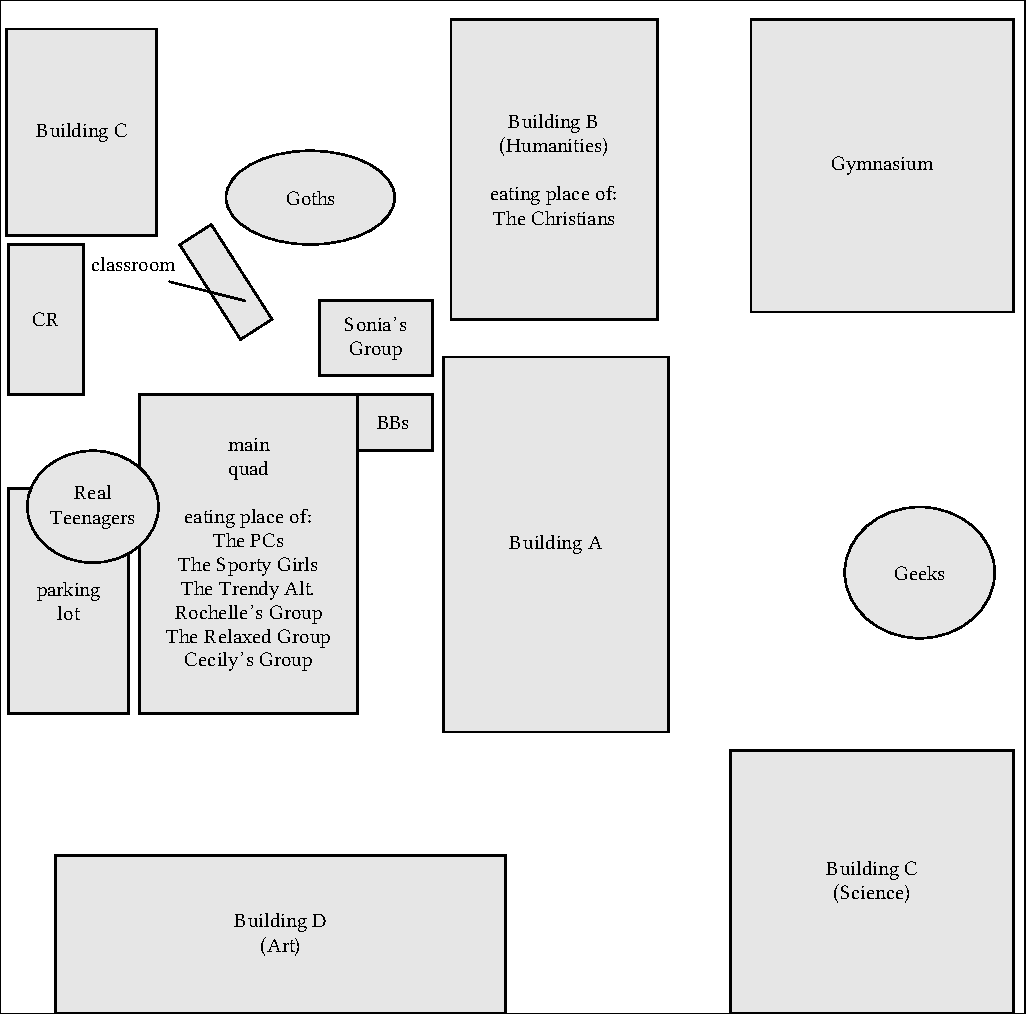
\includegraphics[width=\textwidth]{images/mySGHmap.pdf}
% 		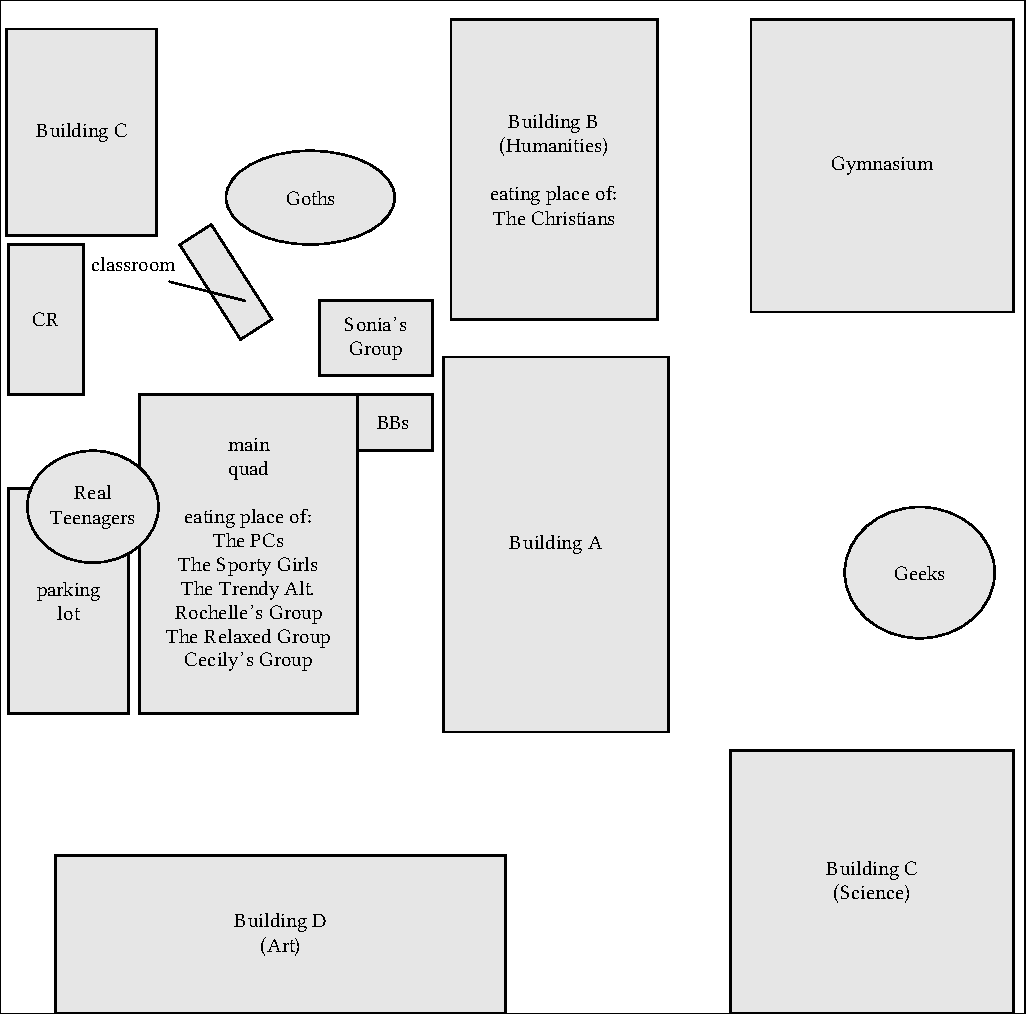
\includegraphics[height=.5\textheight]{images/mySGHmap.pdf}
	\caption{Map of SGH}
	\label{fig:mySGHmap}
\end{figure}


%Some of these group labels, for example \isi{The BBs}, were used by other girls to refer to only one of the sub-groups of a larger, merged group. However, for simplicity, I have adopted the terms to refer to the large, merged groups. 

\tabref{CRNCR} displays the division of the groups into the Common Room (CR) groups and the Non-Common Room (NCR) groups.\footnote{During the Study period, \isi{The Pasifika Group} often used the common room when no one else was there. However, they refrained from using the room when it was full of CR girls (e.g., during lunchtime) and they did not adopt the \isi{norms} of the CR girls. Therefore, these girls have been identified as \isi{NCR girls}.}  These groups will be discussed in more detail shortly.

     
     
\begin{table}[t]
\caption{Common Room (CR) and Non-Com\-mon Room (NCR) Groups, in the or\-der in which they are dis\-cussed}\label{CRNCR}
	 \begin{center}
		\begin{tabular}{ll}\lsptoprule
	
CR&NCR\\
	\\ \midrule
\isi{The PCs} & \isi{The Pasifika Group}\\
\isi{The Sporty Girls} & \isi{The Goths}\\
\isi{The BBs} & \isi{The Real Teenagers} \\
\isi{The Trendy Alternatives} & \isi{The Christians}\\
Relaxed Group & \isi{The Geeks} \\
Rochelle's Group & Cecily's Group\\
 &  Sonia's Group\\
 & Loners \\

\lspbottomrule
		\end{tabular}
	
	\end{center}
\end{table} 

\subsection{CR groups}
\label{group:CR}

The differences between CR groups were more subtle than those found between the \isi{NCR groups}. In general, girls in CR groups took part in school activities and played sport. They represented a mainstream P\=akeh\=a (New Zealand European) sense of style. Being prude or dressing differently than the other CR girls was not considered acceptable. They wanted to be liked and they wanted to be admired. CR girls conformed to each other in what they liked and what they did, thereby setting the \isi{norms} of the school. In some sense, they controlled, or at least embodied, the expectations of the school and of mainstream P\=akeh\=a society.

In the following sections, I describe the different groups who ate lunch in the CR. For a complete list of names of girls in each group, please refer to Appendix \ref{app:socialgroups}. Throughout the chapter, I refer to particular girls as the central/main member, a core member, or a fringe member. This is based on my observations of the groups and the information gleaned from conversations, such as which girls were named when describing both their own or another group. They were not labels used by the girls but are meant to give the reader an idea of the social make-up of each group.

\largerpage
\subsubsection{The PCs}
In addition to observing the groups, I asked the girls about what different groups there were at the school. When questioned, they almost always first mentioned \isi{The PCs}. The term ``PC'' refers to The Palms Crew, The Palms being a popular mall in Christchurch that the girls frequented. Girls from other groups admitted that they also sometimes shopped at The Palms, but the group had been labelled in junior years when \isi{The PCs} were the only group who hung out at the mall.

Non-PCs explained that in order to be a PC, a girl had to be good-looking. As an outsider to the school, it seemed less that \isi{The PCs} were inherently more beautiful than girls in other groups, and more that they wore the season's latest fashions from Christchurch's trendiest shops. While all PCs wore trendy clothes outside of school, only some members of \isi{The PCs} straightened their hair and wore make-up and trendy clothes to school. \isi{The PCs} who did not follow this trend went to the other extreme, wearing old track pants with holes and sometimes not brushing their hair. One of these girls, Kendra, explained that she didn't see the point of trying to look cute at school because there was no one she was trying to impress. Outside of school, however, she adopted the trendier styles of the other PCs. 

Talking with Glenda (\isi{The BBs}) and Ursula (a foreign exchange student who had joined \isi{The BBs}), it became clear that \isi{The PCs} were popular, not in the sense that they were the most liked, but in the sense that other girls looked up to them as the definers of what is and what is not fashionable. \isi{The PCs} were also sometimes referred to as The Plastics, a reference to characters in the Lindsey Lohan movie Mean Girls because they were known to be ``fake''\footnote{According to Urban Dictionary (urbandictionary.com), \textit{fake} is a term used to describe a person, usually a girl, who ``acts too nice to be real in order to lure in pathetic dopes and use/betray them, frequently crushing the victim's soul in the process.''  For more detail, see work by Stacy Lewis, who has conducted a linguistic analysis of ``mock fake'' speech: speakers imitating girls who are fake \citep{lewis2007}.} and to talk about each other behind each other's backs. When Ursula first came to SGH, she ate lunch with \isi{The PCs}, but she switched groups because she said their conversations made her feel uncomfortable. Both Glenda and Ursula were quick to add that, while as a group they did not particularly like \isi{The PCs}, each of \isi{The PCs} was nice on an individual level. I wondered whether this was related to the Losers Sit Alone rule: individual PCs being nice when interacting one-on-one because they did not want to be seen alone. Whether or not this is true, \isi{The PCs} were not the most well-liked group at SGH, but they were certainly the most popular.

%A number of \isi{The PCs} had jobs (several worked at the mall), and most of the central members of \isi{The PCs} lived in upper class suburbs and received money from their parents.

Neither Cleo nor Kim (\isi{The PCs}) were especially forthcoming with me and both eventually refused to take part in further interviews. Kendra, however, encouraged me to spend time with her group, explaining that I would get crazier stories from them than from any of the others. She was not entirely incorrect. Members of this group threw large, exclusive parties and they openly discussed sex, alcohol, and party pills. Noelle, June, and Joanna did fairly well in school, but the majority of \isi{The PCs} viewed school as a social arena rather than a learning centre. In fact, by the end of the year, Marilyn, Amber, Larissa, Kendra, and Minnie had dropped out. \isi{The PCs} who stayed until the end of the year expressed a mixture of excitement and sadness when graduating; they worried there would never come a time when everyone in their group was together again. As Tracy lamented, ``I think I need another year'' (Tracy, \isi{The PCs}, Interview, 22-10.)




\subsubsection{The Sporty Girls}
\isi{The Sporty Girls} were active in the school, though many of them had been more involved in previous years. Though distinct groups at the beginning of the year, contact between \isi{The PCs} and \isi{The Sporty Girls} increased as the year progressed. There were two groups within \isi{The Sporty Girls} who were especially close: Stella, Candice, Rachel, Elise, and Naomi; and Stella, Patricia, Ruby, and Betty. Stella is listed in both groups because she appeared to be the uniting member between them. Patricia's closest friends went to other schools, but at SGH her closest friends were Stella and Ruby. Kanani joined the group at the beginning of the year. She was the only girl in the study who switched from a NCR group to a CR group.\footnote{In terms of the production patterns that are presented in Chapter \ref{ch:prod}, Kanani behaved more similarly to the \isi{NCR girls} than the CR girls. Though I have not yet examined other features of her speech systematically, she appeared to use a mixture of phonetic features utilised by girls in both groups.}

Girls in the group viewed themselves as friendly, ``normal'', and ``in between''. The label, \textsl{Sporty}, was not something used by the girls in the group to refer to themselves. Though some of them wore athletic clothes to school, sports were not necessarily how they identified. In fact, Patricia did not play sport at all and, along with Betty and Ruby, wore some of the trendiest clothes of all the girls. \textit{Sporty} was a label used to refer to this group by girls in other groups, most likely as a result of the clothing worn by Candice, Stella, and Rachel. At the beginning of the year, Naomi also wore athletic clothes, but by the end of the year she had switched entirely to wearing trendy clothes and make-up.


\subsubsection{The BBs}
\sent{

Pam and Odette (\isi{The BBs}). Fieldnotes, 06-04.
\vspace{3 mm}

Pam:		the PCs may be cooler than us

Odette:	but we'll go further in life

}\label{ex:pamodette}

\vspace{5 mm}
 
\noindent Although girls in their final year at Selwyn Girls' High were no longer required to wear a uniform, some members of \isi{The BBs} continued to wear theirs, thereby acquiring the label ``the Blazer Brigade''. This was a friendly group of girls who were good students and who participated in a large number of school activities. At the beginning of the year there were two distinct groups, one of which was referred to as \isi{The BBs} and the other of which was referred to as Pam's group. Upon recognising that they were really very similar, they began to spend more time together and, by the end of the year, had merged into one group. I use the term ``BBs'' to refer to the ultimate, larger group. 

%[[Most of \isi{The BBs} are native speakers of \isi{NZE}. Glenda, however, spent her childhood in Australia and came with her family to NZ for \isi{high school}.

%Star, Madison, Pam, Natasha and several others were popular among the girls at Selwyn High, and in general, the group was well-liked. Priscilla, however, was not. CR and \isi{NCR girls} alike disapproved of her announcements of high marks on assignments, especially when her claims were proved untrue. Unfortunately, I had very little interaction with Priscilla as she was rarely free during study or breaks. When I commented on her busy schedule, she explained that she had many causes that kept her busy, and the school still expected her to do more. However, she continued to take part in causes she was less than enthusiastic about because if she didn't do it, who else would? ]]- REMOVE?  TMI?? 

Most BBs were friendly with girls from a number of groups, particularly those who also ate lunch in the common room. They were talkative in class and were involved in school activities. They went to parties and several of them were sexually active. They were more subdued than \isi{The PCs} in how they partied and they were less inclined to discuss details of parties with me. 

\isi{The BBs} viewed themselves as ``normal''. As shown in Example \ref{ex:pamodette} above and Example \ref{ex:notsupercool} below, \isi{The BBs} viewed themselves as somewhere in between the other groups. They were good students, but they did not view themselves as geeks.

\sent{
Andrea (\isi{The BBs}). Interview, 31-07.

\vspace{3 mm}

Andrea:   we're not like super cool \newline
					but we're not . like . super nerdy 
					
					[laughter]
					
					if that if that's that doesn't sound too mean

}\label{ex:notsupercool}

\vspace{5 mm}

They were school-oriented and felt a responsibility to be good role models for younger girls. They were friendly toward girls in other groups and Andrea claimed that they got along with other groups better than anyone else did. \isi{The BBs} who did not wear their uniform wore casual clothes, such as jeans and a t-shirt, and most of the girls planned to attend university. 


\subsubsection{The Trendy Alternatives}
\isi{The Trendy Alternatives} were artsy girls who took the latest trends and put a twist on them. The girls effectively treated Justine as the leader of the group and she was freely able (and willing) to interrupt the conversation and determine its direction.

Justine described university-bound students from other groups as ``the people that wanna do something with their lives'' (Justine, \isi{The Trendy Alternatives}, Interview, 03-05), but she did not feel the need to succumb to society's expectations of attending university directly after \isi{high school}. Though some girls in \isi{The Trendy Alternatives} were not particularly interested in school (e.g., Justine and Jewel), they planned to go to university after the age of twenty, at which point universities in New Zealand do not have entrance requirements. Other girls in this group were more school-orientated (e.g., Pascal) and went straight to university after \isi{high school}. 

\largerpage[-1] %longdi\isi{stance}
Although this group often ate lunch in the common room, they rarely spoke to girls from other groups. Kelly and Clementine were exceptions. Although they did not sit with other groups (and were therefore not viewed as traitors), they sometimes interacted briefly with \isi{The BBs}. Kelly was well-liked by girls in other groups. Lily, who expressed feeling like an outsider to her own group, was also friends with Rose (\isi{The Relaxed Group}) and Kanani (\isi{The Sporty Girls}), but she quickly left their side if someone from her own group walked into the room. Justine was on the committee that was planning the formal, as were a number of other CR girls. She had a clash with several girls from other groups over the venue for the formal. She was accused of being too outspoken on the subject and was reluctant to argue with them because she did not want to appear ``outspoken about being accused of being outspoken'' (Justine, \isi{The Trendy Alternatives}, Fieldnotes, 13-04).

%Other than Lily, this was a tight group who often met up together outside of school. On one occasion, they went to dinner at Tandoori Palace, an Indian restaurant in town, after which they split into two groups and tried to see how many times they could take the glass elevator in the Crowne Plaza. (In the end, only one group, who went up twice, was successful; the other group had a run-in with a security guard.)

\subsubsection{The Relaxed Group}\label{relaxedgroup}

Rose and Megan were the two central members of \isi{The Relaxed Group}.\footnote{Girls referred to this group as ``Rose's Group''.}  They were best friends and they had been since primary school. The group was also made up of Barbara, Katrina, Lorna, and Anita. Anita transfered to SGH at the beginning of the year. I met her just before the school's powhiri, a traditional M\=aori welcome ceremony which served to welcome new guests to the school grounds. She had just been approached by Rose and Megan, who, upon seeing me trying to figure out where I was meant to go, suggested that Anita and I stick together. Although shy and understandably confused by my role as a researcher rather than a student or teacher, Anita befriended me immediately. She also joined the group of the very first girls she met at the school. This was a group with whom I also felt comfortable and I often sought them out. Rose became one of the girls with whom I was closest and we have continued to stay in touch, nearly ten years since my first day at SGH.

While most of the girls in this group agreed that having fun was what life was all about, Katrina had a different outlook. She expressed frustration at being a teenager and she felt a great deal of pressure from her parents and the school, lessening her enjoyment of the life that her friends seemed to cherish. The other girls felt responsible to look after Katrina. This sense of responsibility was so strong that it tarnished the fun of the formal. Katrina did not want to attend, but her friends insisted that she come. She had a fight with her Mum just before the formal started and she spent the night distant and upset, sitting at the table with me rather than with her friends, and remaining there with my date when girls grabbed me to go dancing. Rose was emotional that night, worrying over Katrina. In general, Katrina was disappointed in Year 13, which she had been assured would be the best year of \isi{high school}. She was not impressed with \isi{high school} and felt ready for the next chapter of her life.\footnote{Katrina was much happier once she went to university. She has made good friends and she now admits that in \isi{high school} she would have liked to have been better friends with \isi{The Goths} but worried at the time that it would cause problems with girls in \isi{The Relaxed Group}.}  

%[it's kind of like there's \isi{youth culture} and then there's human beings [Katrina on being treated differently by adults - biancakatrinacandice18sept.trs]]  

When I asked Megan and Anita what made their group different from other groups, they explained that they were more relaxed and cared less about image than some of the other groups. They explained how they could wear jewellery or a belt if they wanted to feel cute one day but that they did not feel pressure to do so if they were not in the mood. Girls from this group wore little make-up to school and their style of clothing was the least trendy of all the girls who ate lunch in the CR. Barbara and Katrina played sport and Rose and Megan became increasingly interested in parties as the year progressed. Lorna was a fringe member and was also good friends with Rochelle's Group.

\subsubsection{Rochelle's Group}
At one point in the year I was struggling with my own personal relationship woes and girls in a variety of groups were exceptionally sensitive to my emotional state, for which I was (and continue to be) extremely grateful. One group in particular offered to listen and provide support because, as Camden explained, ``We know drama'' (Fieldnotes, 26-10). And indeed, these girls did. From break-ups to break-ins, these girls almost seemed to thrive on their struggles and the mutual fondness they gained through sharing their stories with each other.\footnote{Because of this drama, I have referred to this group elsewhere as the Drama Queens \citep{drager2008lsa}. I am not entirely happy with this label: It was not one used by any of the girls and they do not fit my stereotype of drama queens. Therefore, I felt it was misleading and have refrained from using the term here.}

This group was a CR group, but apart from Lorna's friendship with girls in \isi{The Relaxed Group}, they did not get along with CR girls from other groups. From my point of view, it seemed as though they intentionally instigated confrontations with other girls. Camden (Rochelle's Group) and Lily (\isi{The Trendy Alternatives}) openly talked badly about one another and Lorna (Relaxed Group/Rochelle's Group) rolled her eyes if one of \isi{The BBs} approached to ask her opinion on a Year 13 matter. Mindy, however, was quiet and friendly both in and outside of class and Rochelle made an effort to be friendly and to smooth things over with other groups. Perhaps it was she, the leader, who maintained their status as a CR group. She was the only one in her group who embodied the CR girls' trait of wanting to be liked and wanting to be admired.
 
Interestingly, these girls performed drama differently from other people I know. Rather than talking up their news as though it was full of juicy details, these girls downplayed their drama. My impression was that they wanted me to believe that they had so much drama in their lives that something that I might consider drama-worthy was hardly worth mentioning. For example, one day when I was talking with both Camden and Rochelle, Camden told me that she thought she was pregnant and that the father was neither nice to her nor wanted to be in a relationship with her.\footnote{She later found out that she was not pregnant.}  Rochelle, an incredible optimist on a number of occasions, stated with a sigh that she wanted to go ice skating and Camden agreed that ice skating would be fun. They were not avoiding the topic of pregnancy; both girls were quite open about sharing this type of information with me. The nonchalant manner in which the information had been provided and the quick change of subject to something entirely unrelated and, in my opinion, much less dramatic, left the impression that dramatic events were so commonplace in the lives of these girls that it hardly needed mentioning. That Camden explicitly made a claim on drama (``we know drama'') indicates that this was in fact the defining characteristic of this group and reflected how they viewed themselves.

%Other girls referred to this group as ``Rochelle's Group'' or sometimes ``Rochelle and Camden's Group''. , and the term ``Drama Queens'' is used because of Camden's claim on drama. Camden made this claim explicitly (``we know drama''), and she  Camden continually shared details of the drama in her life, both with her friends and with me. 

\largerpage
\subsubsection{CR groups as a constellation}
  
The CR girls' claim on the common room was no coincidence. The common room was a piece of prime real estate and they felt entitled to use it. Through actions such as writing on the whiteboard and posting photos of their friends on the wall, they not only used the room but made sure everyone knew that it was theirs. They believed, or at least claimed to believe, that everyone was friends with everyone else. If everyone was friends, there was no need to negotiate who was entitled to use a shared space like the common room.

Together, the groups who ate lunch in the common room formed a \isi{constellation of practices}, a term used by \citet{wenger1998} to refer to groups who were too broad and diverse to be considered communities of practice but who shared interconnected practices nonetheless. ``The term \textit{constellation} refers to a grouping of stellar objects that are seen as a configuration even though they may not be particularly close to one another, of the same kind, or of the same size'' \citep[127]{wenger1998}. He explains that constellations of practices are more abstract than communities of practice.  They need not be named nor do the individuals need to be aware that they form any kind of grouping. Though between CR groups there was a web of interconnected practices, they did not form the tightly woven bonds of a community of practice as described by Wenger. The CR girls were not the only \isi{constellation of practices} at the school. The whole of Year 13 was a \isi{constellation of practices} and, in fact, the whole of Selwyn Girls' High was as well. Constellations of practices can take a number of forms and can be observed at multiple levels of categorisation.

The CR girls also formed what I refer to as a \textit{constellation of stance}, an aggregate of individuals or groups of individuals who commonly take shared stances toward other individuals, concepts, and constructs. It is this that sets them apart within the constellation of the school. Here, I take \isi{stance} to mean ``a socially recognised disposition'' \citep[2]{ochs1990}. CR girls expressed similar views of themselves and similar attitudes toward these views (e.g., the view that they were ``normal'' and that ``normal'' was a positive attribute, that upward social mobility was a positive attribute and that people who did not aim for it were not going to go far in life). Through doing so, they form a constellation of \isi{stance} and they shared a number of interconnected practices (e.g., planning the formal, playing sport, and going to parties), thereby forming a \isi{constellation of practices}. The reason behind distinguishing between these different types of constellations will be clearer in the following section which discusses the \isi{NCR girls}: While the \isi{NCR girls} formed a constellation of \isi{stance}, they did not form a \isi{constellation of practices} that was separate from that which they also shared with the CR girls.

  

\subsection{NCR groups}
\largerpage[-1]
Despite the CR girls' claims, not everyone at SGH was friends with everyone else. There were girls who were not accepted into CR groups but who, for the most part, did not want to be. Though the groups shared little in common with one another, \isi{NCR groups} actively rejected the behavioural \isi{norms} set by the CR girls, and, in doing so, unwittingly shared a common \isi{stance}. 
 

Of course, the different \isi{NCR groups} each established their own sets of \isi{norms}. For example, girls in \isi{The Real Teenagers} were expected to party and girls in \isi{The Geeks} were expected to try hard in school. But the number of members in each of the groups was simply not high enough to overturn the school's \isi{norms} set by the CR girls. In other words, while there were \isi{norms} for each of the \isi{NCR groups}, they were not the \isi{norms} of the school.

\subsubsection{The Pasifika Group}

All members of \isi{The Pasifika Group} were M\=aori or Pacific Islander (PI).\footnote{Pacific Islander is a term used to refer to people with ancestry from Polynesia, Micronesia, and Melanesia. In New Zealand, it is does not usually include indigenous New Zealand M\=aori.} While there were M\=aori girls in other groups, ethnicity was not a topic they introduced into our conversations.\footnote{One exception was Kanani, who was proud of her Polynesian roots but distanced herself from \isi{The Pasifika Group} after switching to \isi{The Sporty Girls}. Girls in \isi{The Pasifika Group} were no longer friendly to her and she constructed her own sense of style (both linguistic and non-linguistic) that was reminiscent of both Pacific Island style and a style consonant with that of her new group.}  Girls in \isi{The Pasifika Group}, on the other hand, immediately identified themselves in terms of their ethnicity and expressed pride in their culture as well as frustration at the lack of ethnic diversity among the students and teachers at SGH and in Christchurch in general. They were particularly frustrated that the school did not seem to address their need for a more ethnically diverse faculty. There was no Pacific Island teacher and they felt misunderstood by the single M\=aori teacher at the school.  The school's failure to hire non-P\=akeh\=a teachers may well be due to a shortage of such teachers, but it left the girls feeling unsupported, as exemplified in Example \ref{ex:don'ttakeseriously}.
  
			
%Masina:  like for us brown people you know . PIs and Maoris . I mean they seem to lift I'm not being racist or anything . but you know they they just seem to lift like . other people . they believe they can do . better than us


\sent{
Masina, Alana and Lela (Pasifika Group). Interview, 20-09.

\vspace{3 mm}

Masina:  'cause I seen it happen quite a lot of times \newline
				but I mean a lot of parents have come in school . \newline
				um . to complain about it but they just .

Alana:  don't take . any notice of it

KD : really?

Lela : yeah it's ``oh yeah I don't care''

Masina: they don't take us seriously

}\label{ex:don'ttakeseriously}

\vspace{5 mm}

%[maybe this one isn't really needed and could be bad if someone at the school read it?]
%\sent{
%Marama:  		There's Miss [The only M\=aori teacher, name removed] 
	%					but she doesn't really know

%Lela : 			but . she doesn't really understand what . you know

%Masina: 		she's a beep [laughter] na honestly like 
		%				oh . she's nice and all but .

%Marama: 	na she's kind of a bitch
%}\caption{Marama, Masina, and Lela, Pasifika Group, 20-09}\label{ex:maoriteacher}

%\vspace{5 mm}

\noindent As demonstrated in Example \ref{ex:weneedsupport}, Masina and her friends felt as though they were treated differently, not by the other girls, but by the school itself. 

\sent{ 

Masina (Pasifika Group). Interview, 20-09.

\vspace{3 mm}
 
Masina:  but . yeah . um I mean they seem . \newline
					like they've had issues with . us brown people um .	\newline
					not attending school and stuff 		\newline
					and they just knock . all of us off . \newline
					like . all that like . one after one they h- \newline
					they're just like . completely give up on us \newline
					instead of giving us the support that we need to stay in school 
}\label{ex:weneedsupport}				
					
\vspace{5 mm}

\noindent They attributed the difference to the colour of their skin, explaining that most of their group had already left school and that they believed that teachers had ``written off'' those who remained. They also viewed themselves as different from the majority of girls, stating that they needed different kinds of support than other girls and wishing that there was a faculty member who understood where they were coming from culturally. They felt that while the school treated them differently, it did not treat them differently in a constructive way.


%Of the girls in \isi{The Pasifika Group}, I became most familiar with Marama, largely through attending her Textiles class, and it took some time before the other girls opened up to me. Once they realised that I was interested in them in addition to other groups in the school and that I would not tell their teachers and families about certain aspects of their lives, they began to share feelings of how they were treated differently from other girls at the school, not by the other girls but by the school itself. 

\isi{The Pasifika Group} had very little interaction with Year 13 girls from other groups. They did not eat lunch in the common room and they kept to themselves during class. One of their good friends, Ripeka, was very involved in the school, both with sport and with kapahaka (traditional M\=aori performing arts) and she had friends in other groups. Unfortunately, I was not able to record an interview with Ripeka.

Although girls in \isi{The Pasifika Group} had little interaction with girls from other groups in their year, they interacted regularly with more junior girls (who were also M\=aori or PI), which was not something done by girls in most other groups. 

\subsubsection{The Goths}

Only one member of \isi{The Goths}, Santra, wore black clothes and dyed her hair black, but girls in other groups referred to the entire group as \isi{The Goths}.\footnote{Goths are a youth subculture that see beauty in the dark side of life. They tend to wear black clothes, heavy eyeliner, and medieval-inspired clothing.}  All of the girls in this group described themselves as ``weird'' and they at least claimed not to care about what other people thought about them. They were intelligent girls who were enthusiastic students but who also questioned the school's ability to teach them life's most important lessons. They were knowledgeable about world events and had strong opinions about societal issues. Santra, Vanessa, Meredith, and Marissa were the original members of the group. In Year 12, \isi{The Goths} were joined by Tania (previously of \isi{The Relaxed Group}) and in Year 13, by Bianca, who seen less and less frequently with \isi{The Geeks} as the year progressed.

\isi{The Goths} had a particular area of the school grounds that they considered their own. It was separated by large plants from the courtyard where most of the other groups hung out and it contained a small wooden deck and a large rock. \isi{The Goths} ate there even when the weather was very cold and on rainy days they moved under the enclave of a building nearby. This group had eaten lunch in this area since the beginning of \isi{high school}. They were very territorial and girls from other groups rarely challenged their claim. However, there was one lunchtime where \isi{The Goths} had to assert their authority. They arrived to the area later than usual and some younger girls were sitting on the deck. Rather than approaching them and telling them to leave, \isi{The Goths} surrounded the deck and exclaimed in loud voices, ``Don't you hate it when people sit in their [sic] spot'' (Santra, \isi{The Goths}, Interview, 03-05). The younger girls gathered their things and left, glaring and mumbling in angry voices under their breath. Girls in \isi{The Goths} tended to be friendly, but the area where they ate was a part of how they constructed their \isi{identity}. They felt they had a claim on the place and they were willing to chance confrontation in order to preserve that claim.


\subsubsection{The Real Teenagers}

Some groups trusted me immediately. I was a researcher and university student. My presence had been approved by the school principal and this legitimised me in the eyes of some students (e.g., \isi{The BBs}). In contrast, it required more work to gain a \isi{rapport} with \isi{The Real Teenagers} and after over a month at the school, I began to lose hope that I ever would. One day, however, the opportunity arose.

``No entry''. The sign on the door was in clear view and it had not been there the day before. I did not know any way to the classroom other than through that door or through a maze of already-full classrooms. I had not seen Onya walk through the door, but I knew she had. Alex was walking toward it.\footnote{At the time, Alex and Onya were good friends. However, once Isabelle switched groups, Alex switched back to Cecily's Group, informing me that it was her ``real group'' while Onya stood listening nearby. Onya (\isi{The Real Teenagers}) and Cecily (Cecily's Group) did not get along though they had friends in common including Alex as well as others who did not go to SGH.}  She opened the door and moved aside the chairs meant to block the entrance, beckoning for me to follow. I hesitated a moment, unsure of whether I should follow this group of rather rebellious girls whose favour I had been attempting to gain (unsuccessfully), or follow my inclination to obey school authority. My desire to abide by the school rules was strong, perhaps a habitual remnant leftover from my own school days, or perhaps out of fear of losing the privilege of conducting research at SGH. The door, having been left unattended while I stood watching it, was just about to close, when suddenly I grabbed it and walked in. While I was maneuvering around the chairs that blocked my way into the hall, the teacher (whose class I had hoped to attend) emerged from her classroom. She glowered and reprimanded me. I felt ashamed and humiliated. Alex came to my defense, at which point the teacher began to aim some of the accusations at her. Alex and I both remained silent, neither of us informing the teacher who, besides myself, had walked through that door.

The shame I felt during the teacher's scolding surprised me. The reprimand itself was not what was surprising; I knew that I had disobeyed the rules and that I deserved to pay the consequences. I was surprised by my shame. 

But if shame was my payment, my reward was \isi{rapport}. From that day forward, this group of girls welcomed me to join them and they openly shared details of their personal lives to a level I had not anticipated. It was then that I appreciated the value of gaining \isi{rapport}, even when achieved through somewhat uncomfortable means, as exhibited by Geertz when he was finally able to gain \isi{rapport} with Balinese locals after siding with them during a government break-up of an illegal cockfight (Geertz 1973). Like Geertz, I had to face the temporary disfavour of an authority figure, but in turn I was able to gain the trust of those with whom I had previously had none. 

\nocite{geertz1973}

\isi{The Real Teenagers} were a group of rebellious girls who partied hard and, as they saw it, lived life to the fullest. One of the core members, Onya, gave an overview of their conversation topics: sex, drugs, and rock `n' roll. \isi{The Real Teenagers} claimed that they didn't care what others thought about them, but the explicit nature of the conversations and the volume at which they spoke while within listening di\isi{stance} of other girls suggested otherwise: They were out to shock. When in class two of \isi{The BBs} said that they wished their lives were as exciting as \isi{The Real Teenagers}', Alex and Onya laughed. They enjoyed their status as the crazy party girls and they were pleased when the other girls acknowledged it.

\largerpage
Most girls at SGH referred to this group as Onya's group; the ``Real Teenagers'' was not a name used by girls at the school. Toward the beginning of the year, Isabelle (formerly of \isi{The Goths}) decided to switch groups. Example \ref{ex:realrealteen} displays a conversation between Meredith, Vanessa (\isi{The Goths}) and me. 

\sent{
Meredith and Vanessa (\isi{The Goths}). Interview, 03-09.

\vspace{3 mm}

KD: how come Isabelle switched groups?

Meredith: to become a teenager

Vanessa: that was her words \newline
to become a teenager
 
KD: what's that mean?

Meredith: the group she's now with \newline
they go out and they get pissed like . every like . \newline
a couple times every weekend \newline
oh they just do stupid things

Vanessa: they have sex a lot

Meredith: yeah have sex a lot they just . \newline
they're like the real real real teenagers

}\label{ex:realrealteen}

\vspace{5 mm}

\noindent The central members of \isi{The Real Teenagers} were Onya, Claudia and Renee. Sarah was also a good friend, though she did not always get along with Onya. At the beginning of the year, Alex (Cecily's Group) and Onya spent a great deal of time together. However, Isabelle, rather than Alex, became Onya's close friend part-way through the year when Isabelle started dating Onya's good friend, Luke. Sally (Cecily's Group) became good friends with Renee over the course of the year but was rarely seen with the rest of \isi{The Real Teenagers}.

Though \isi{The Real Teenagers} and \isi{The PCs} shared a love for parties and a less than enthusiastic outlook toward academic subjects, the groups were different on a number of counts. \isi{The PCs} had values associated with more mainstream New Zealand society. Many of the girls belonged to higher socioeconomic groups and PCs who did not live in prestigious suburbs (e.g., Fendalton or Sumner) didn't talk freely about the area where they lived. \isi{The PCs} wore clothes from chain stores found at New Zealand malls. They wanted to be liked by girls in other groups and they smiled at girls who they talked badly about afterward. In contrast, \isi{The Real Teenagers} rejected mainstream values in favour of a more artistic chaos: homemade skirts accented in ribbons and lace, worn with Doc Marten boots, fishnet stockings, and handmade accessories from the clothing boutique where Claudia worked. Though high heels were not allowed at school, Onya loudly clomped down the main corridor wearing heels in defiance. Many of the girls belonged to lower socioeconomic groups. Onya talked with pride about living in Aranui, the poorest and most stigmatised suburb in Christchurch, and Renee explained that she had only brought a banana for lunch because her father couldn't afford the groceries that week (at which point her friends divvied up their lunches and shared them with her). They wanted other girls to recognise their party lifestyle and they wanted to be admired, but not for their money or their parents' social status. And they displayed no desire to be liked; they made it perfectly clear to all when there was someone they did not care for.

\subsubsection{The Christians}

In stark contrast to \isi{The Real Teenagers} were \isi{The Christians}. This group was made up of two girls: Esther and Theresa. Esther and Theresa felt most comfortable among people who shared their beliefs and adhered to their expectations of right and wrong. Despite their general satisfaction with life, they felt separated and different from the other girls at the school. Both worked hard at school and expressed enjoyment of their adolescent years.
 
Theresa, who was not religious prior to meeting Esther, grew up in a small rural town in New Zealand and Esther spent her childhood in a small village in France. They became good friends after Esther invited Theresa to Easter Camp, a multi-day Christian camp with live music, games, and activities. At the time, Esther had only lived in the country for a short time and had not realised that there were non-Christians in New Zealand. She invited Theresa assuming she would already be familiar with the idea of Easter Camp. Theresa came out of curiosity and had a wonderful time surrounded by more people than she had ever seen. Esther and Theresa were best friends from then on. 

Both Esther and Theresa dressed conservatively and said they would not feel comfortable wearing clothes, such as short skirts, that many of the other girls wore. Like girls in \isi{The Pasifika Group}, they interacted very little with other girls in their year but had several friends from youth group who were in more junior years. Exceptions in Year 13 were two of \isi{The Goths} with whom they occasionally interacted during Study, though only one of \isi{The Goths}, Marissa, encouraged the friendship. Both Esther and Theresa were good students and had conservative values and they both viewed Christianity as the defining feature of their group. There were other Christians at the school, but it was viewed as a characteristic of an individual as opposed to the central component of the group's \isi{identity}.
 
\subsubsection{The Geeks}\label{geeks}

The girls in this group did not fit my stereotype of ``geek'' at all. I viewed them as an eclectic group of individuals, each with their own distinct style. It was the most multi-national and multi-cultural group in Year 13. ``\isi{The Geeks}'' was a label used by other girls to refer to this group; it was not something used by the members themselves. Although this was not a group commonly mentioned by girls in other groups, CR girls used the term ``Geeks'' when asked explicitly about the group. 

The make-up of \isi{The Geeks}, most of whom were good students, only formed in Year 13. Joy, who was originally from Australia, attended another school in Christchurch before coming to SGH in Year 12. In intermediate school\footnote{Intermediate school is between primary and secondary school and is equivalent to junior high or middle school in countries such as the United States.}, Mariah had been in a group with some of \isi{The BBs}, but that group broke up when the unifying member moved to Australia. Valentina was new to SGH but quickly became a core member of the group. Aerial had a falling out with her former group (\isi{The Relaxed Group}) the previous year and \isi{The Geeks} befriended her. Bianca, a fringe member of \isi{The Geeks}, also spent time with \isi{The Goths}, and by the end of the school year was spending more time with \isi{The Goths} than with \isi{The Geeks}. 

On warm days, most girls at SGH ate lunch on the sunny side of the school. \isi{The Geeks}, however, ate lunch on the other side of the building from the main quad, as shown in the map in \figref{fig:mySGHmap}. The only other groups who ate in this area were in younger years. Joy and Mariah, the two central members, tended to dominate the lunchtime conversation. 

The styles worn by \isi{The Geeks} varied more than those worn by girls in other groups. For example, Aerial and Valentina wore short skirts and sandals, while Joy wore track-pants; Aluna and Nisha wore long flowing skirts, Kristin wore punk clothes with studded wrist bands, while Mariah wore corduroys and blouses from secondhand shops. Though styles of apparel varied among \isi{The Geeks}, girls from other groups saw fit to comment on their clothes, particularly those of Joy, Kristin, and Mariah. The other girls' expectations of what the girls in \isi{The Geeks} should wear were not the \isi{norms} of the school; \isi{The Geeks} were expected to dress differently from the other girls. For example, one day Mariah came to school wearing a purple nose ring. The other girls were shocked, telling Mariah that it didn't suit her. Megan (\isi{The Relaxed Group}), who was critical of Mariah's nose ring, had a lip ring herself and had commented on how she liked my nose piercing. It was not as though the girls did not accept piercings in general; they did not accept that Mariah, a Geek, would pierce her nose. After nearly an hour of taunting, Mariah removed her nose ring, revealing that the nose ring was one that did not require a piercing and that her nose was not, in fact, pierced. The other girls teased her even more after realising that the piercing wasn't real and Mariah never wore the purple nose ring to school again. 

%\footnote{I never heard anyone comment on clothes worn by Aerial or Valentina, despite their style being similar to that of \isi{The PCs}. A possible interpretation is that Aerial was once a CR girl, and it was acceptable for her to wear trendy clothing despite no longer being friends with the CR girls. Valentina, who was from South America, had a slightly different style, and the girls may have assumed and accepted that she dressed in a manner appropriate to where she was from.} 
%The geek girls resisted the comments for only a short time, eventually \isi{conforming} to the other girls' expectations of what they should wear. 
%By the end of the year, most of the girls had tried either beer or vodka at least once, but they did not party frequently. 

\subsubsection{Cecily's Group}

Cecily's Group was a group of friendly and funny girls. They had an alternative sense of style and liked live music and art. The majority of girls in Cecily's Group took art classes and several of them played musical instruments. Their interests were diverse and Sally explained how they each had their own little niche within the group through these different interests. Sally was an artist, Pania was a surfer, and Lindsey was a Christian, but they all enjoyed doing things together and valued each other's friendship.

When I asked Sally whether she thought the school was very divided, she first claimed that most people at the school got along but then added that there was some level of judgment by at least some people, as shown in Example \ref{ex:sallyjudges}.

\sent{
Sally (Cecily's Group). Interview, 11-04.

\vspace{3 mm}

Sally:	everyone just goes and has fun like

KD: yeah

Sally: 	I don't know . \newline
				but maybe slightly judgmental sometimes I don't know \newline
				there's some degree of judgment everywhere I suppose eh

}\label{ex:sallyjudges}

\noindent As discussed in Section, \ref{sec:salience}, the belief that everyone ``just goes and has fun'' is consistent with the \isi{stance} of the CR girls, whereas acknowledging that some girls are judgmental is consistent with the beliefs of the \isi{NCR girls}. This suggests that Sally's views were somewhere in between those of the CR girls and the \isi{NCR girls}.  In fact, the girls in Cecily's Group seemed to get along with girls in \isi{NCR groups}, such as \isi{The Real Teenagers}, as well as CR groups, like \isi{The BBs}. 

Members of Cecily's Group were good students, but they also partied and they genuinely seemed as though they didn't care to (or feel the need to) meet the social expectations of the CR girls. Cecily appeared to be the most central member and was usually the girl mentioned when other girls referred to this group. Because the girls in Cecily's group were very active at the school and had little free time, I had less of a chance to get to know them as well as I would have liked. 


%\subsubsection{Art Room girls}

%The Art Room girls formed a group of close friends who were active at the school. In many ways, they were similar to \isi{The BBs}, and in fact they were friendly with \isi{The BBs}. They wore alternative style clothing and were very involved in art class, so much so that they usually spent their breaks working on projects in the art room rather than sit outside with the other students.

%In contrast to the other \isi{NCR groups}, the Art Room girls were friends with a number of people in different CR groups. 


\subsubsection{Sonia's Group}

Sonia's Group was not a group that was pointed out by the other girls.\footnote{Sonia appeared to dominate conversations. Although I am not certain that she was actually the central member, I have used her name in the group's label.}  I came to know two of the girls in this group, Holly and Sonia, through attending their Study period. Though neither of the girls were seen conversing or sitting with \isi{The PCs} at school, Holly and Sonia saw some of \isi{The PCs} on a bus trip one weekend, a drunken night where groups are bussed between out-of-the-way pubs in and around Christchurch. Thereafter, both Holly and Sonia talked about \isi{The PCs} as though they were friends, leaving me with the impression that they looked up to \isi{The PCs}. Given their acceptance of the CR \isi{norms}, this group could potentially be classified as a CR group.\footnote{In the production analysis presented in Chapter \ref{ch:prod}, patterns in Holly's speech more closely resembled those found in the speech of the CR girls. However, I deemed it to be poor methodology to alter my qualitative analysis after this time,  but I interpret Holly's use of both linguistic and non-linguistic factors associated with CR girls to be consistent with her eagerness to conform to the CR girls' \isi{norms}. This is discussed further in \sectref{sec:idconstruction}.}  However, I have listed them here as a NCR group because they did not actually eat lunch in the common room.

\subsubsection{\isi{NCR groups} as a constellation}

The groups labelled here as NCR were a mix of diverse groups with very distinct ideologies and lifestyles. By placing them in a single group (NCR), I do not mean to imply that there were similarities among them. The trait they shared was a rejection of the practices that were established as normal by the common room girls, forming a constellation of \isi{stance}.	``We not only produce our identities through the practices we engage in, but we also define ourselves through practices we do not engage in'' \citep[164]{wenger1998}.

\largerpage
\noindent  The \isi{NCR groups} were separate, diverse groups with wildly different styles from one another, but crucially, they all viewed themselves as different from the other girls. 


\subsection{Outside of lunchtime}

The CR-NCR distinction extended beyond the lunch hour. There was one Study group in particular that exemplified the divide. While most groups in a single Study period were made up of fewer than 20 students, there was one period where over 30 students had Study. Due to the larger number of students, two classrooms (as opposed to the usual single room) were provided and the students were free to chose which of the two rooms they spent the period in. Without exception, girls in CR groups sat in one classroom and girls in \isi{NCR groups} sat in the other. The \isi{NCR girls} interacted minimally across the different groups, though occasionally Esther (\isi{The Christians}) commented on conversations between different members of \isi{The Goths}. The CR girls, on the other hand, sat on top of the desks and talked with one another throughout the Study period.

When running the \isi{perception} experiments, I asked the CR girls in this Study period if they would like to take part. Maya suggested that I ask the girls in the other room, commenting that they would be happy to help and that she would help later if I still needed participants.\footnote{Maya did later take part in the experiment.}  As I walked from one room to the other, I heard the CR girls laughing. I presumed that they were laughing at Maya's dismissal of my experiments, pawning the task off onto a group of girls with whom she did not care to interact. Alternatively, they may have been laughing because Maya told me what to do and I obeyed: I went to the ``others'', thereby acknowledging that they were the ``freaks and geeks'' who would take part in experiments and it was with them that I belonged. 

There was no label used to describe the differences between girls in one room and girls in another, but this is not surprising: Constellations of practices often go unnamed \citep[128]{wenger1998} and I suspect that constellations of \isi{stance} are even less likely to be named. Despite this, Maya had inadvertently acknowledged the divide between the Year 13 groups.



\section{Salience and stance}\label{sec:salience}
The \isi{Second Wave} of variationist studies emphasises the importance of using an ethnographic methodology in order to uncover social groupings of a community that are relevant to the speakers within that community. There is always a danger of a researcher imposing their expectations and prejudices upon speakers, thereby failing to identify categories that are relevant to the individuals being studied. However, I believe that less salient groupings of speakers can also be relevant to sociolinguistic variation. Extending the meaning to the context of SGH, I use the term \textit{relevance} to refer to how much a factor or group is ``connected with, or pertinent to the matter at hand'' (`Relevance' 2002), regardless of whether that factor or group is above or below the level of consciousness. I use the term \textit{salience} to refer to a gradient level of importance or prominence of an item in relation to its neighbours; the more salient an item, the more the item stands out. Salience attracts attention, and greater attention leads to a higher liklihood of \isi{awareness}.

\largerpage[-1]
Although girls at the school were acutely aware of the different, smaller groups (e.g., \isi{The PCs}, \isi{The BBs}, etc.), they were not aware of the constellations of \isi{stance}: the CR-NCR distinction. This is not to say that the girls were unaware of where other groups ate lunch (though several CR girls had trouble naming \isi{NCR groups}), but CR groups and \isi{NCR groups} were not listed as belonging to a shared grouping.  As mentioned earlier, Maya referred to the \isi{NCR girls} in the other room and treated them differently to the CR girls she was surrounded by, but this was the closest anyone came to acknowledging this divide. No one used labels to refer to CR versus \isi{NCR groups} and no one even mentioned the similarities across the different CR groups. The groupings ``CR girls'' and ``\isi{NCR girls}'' were not salient categories at the school and I want to make it clear that I am not arguing that they were explicit categories at all: They were groupings of girls who shared similar stances to the school's \isi{norms} of behaviour. CR girls shared the belief that they were ``normal'' and in doing so, they conformed to each other's \isi{norms}, thereby setting and perpetuating the \isi{norms} themselves. In contrast, girls labeled as ``\isi{NCR girls}'' shared a \isi{stance} that was something akin to different than the norm. They rebelled against the \isi{norms} of the CR girls in different ways (e.g., Santra of \isi{The Goths} wore all black; Esther and Theresa of \isi{The Christians} refrained from drinking alcohol; Joy and Aerial of \isi{The Geeks} sat at the front of the classroom; Marama and Angel of \isi{The Pasifika Group} did not reject their cultural values in favour of the P\=akeh\=a values that were embraced by the CR girls). These acts of defiance of the \isi{norms} served to construct their social personae. CR girls and \isi{NCR girls} formed two separate constellations of \isi{stance}. Consistent with work in the \isi{Third Wave}, I argue that linguistic variables can be indexed to stances rather than to any category of ``CR'' or ``NCR'', thereby allowing linguistic variables to be correlated with abstract groupings of individuals (constellations) of which the speakers themselves are less aware. A linguistic analysis and a discussion of how it correlates with these positions of ``normal'' and ``different'' can be found in Chapter \ref{ch:prod}. Here, I discuss some of the stylistic choices made by CR and \isi{NCR girls} and then I provide several examples of interactions with the girls that help to illustrate their different stances. 

A group's choice of lunch locale symbolises the position taken by those girls who conformed to expectations and \isi{norms} at the school and those who did not. The girls' choice of clothing, piercings, and activities supports this distinction. The CR girls most often wore clothes from chain shops found in malls throughout New Zealand. In most groups there was at least one girl with a facial piercing, usually a lower lip, eyebrow, nose, or Monroe (a piercing that is placed off-centre in the upper lip and resembles a beauty mark). Across the different \isi{NCR groups}, there was a much greater amount of variation in how they dressed. \isi{The Real Teenagers} mixed their own homemade creations with designer ones, and some had multiple facial piercings (e.g., both nostrils and the back of the neck). In contrast, \isi{The Christians} wore conservative clothing and had naked faces (i.e. no make-up or piercings). That girls from the different \isi{NCR groups} did not dress similarly to one another is not surprising. The girls were defined as \isi{NCR girls} not by what they were but by what they were not: CR. Instead of focusing on commonalities between them (of which there were few), I wish to highlight the multitude of identities and the manner in which they failed to conform to the behavioural \isi{norms} established by the CR girls. As individuals, they each rejected the expectations of the majority of girls at the school. Each of the groups rejected the \isi{norms} in different ways, but some of these acts, such as not eating lunch in the CR, were shared across the different groups. Therefore the common room was more than a mere eating place: It reflected the degree to which an individual conformed to the \isi{norms} established at the school.

%In fact, after the last assembly of the year at which I presented the idea of CR and \isi{NCR groups}, a number of girls, particularly CR girls, expressed surprise at the distinction. Is the CR-NCR distinction then a valid grouping, or is it a case of a researcher imposing categories on speakers that are not relevant to the speakers themselves?  I will argue that a grouping need not be completely above the level of consciousness for a particular speech community for it to be relevant for that community and for it to co-vary with linguistic variables.\footnote{Throughout this dissertation, I will use the term `relevance' to refer to importance of a factor that can be either above or below the level of consciousness, and the term `\isi{salience}' to refer to a gradient level of importance or standing out in relation to its neighbours; the more salient an item, the more conscious an individual is of the item. The categorical distinction of above or below the level of consciousness could be based on some threshold within the continuum of \isi{salience}.}  In Chapter \ref{ch:disc}, I will discuss how Exemplar Theory (see Chapter \ref{ch:litrev}), predicts that both phonetic variation and social variation can be below the level of consciousness and still be closely related.


%The girls could easily name who ate lunch where and with whom, but they did not consciously divide individuals into CR and \isi{NCR girls}. Girls were divided at the individual group level, not at the lunch locale level. Although this binary distinction between the groups is not a distinction that the girls were explicitly aware of, it reflects more than a mere eating place. CR girls established and conformed to the school's \isi{norms}, and \isi{NCR girls} walked to the beat of their own drum. 

%The girls who used the common room frequently expressed fond memories of their time at SGH. The memories were not necessarily of the school itself but of friends and amusing events. 

During interviews, CR girls most often commented on how everyone at SGH was friends and how there was not the clear division between groups that they associate with US high schools.\footnote{I suspect this was usually a comment made to me specifically as an American.}  For example, when I asked Rachel what groups there were at the school, she responded,

%Andrea (\isi{The BBs}) describes everyone in Year 13 as ``nice'', and 

\sent{
Rachel (\isi{The Sporty Girls}). Interview, 13-04.

\vspace{3 mm}

Rachel:	like there's . kind of like what everyone calls like \isi{The PCs} and then like \newline
				like little groups and stuff \newline
				but then in a way everyone I feel s- kind of gets on with everyone else as well \newline
				like I don't feel like it's that divided \newline
				well that's how I feel like some people might think it's different \newline
				but I kind of feel like I'm friends with everyone like like 

KD:	that's cool 

Rachel:	I don't feel like I don't have the right to t- go like \newline
		go up to a group and sit down with them \newline
		hang out with them one lunchtime \newline
		or anything like 
}\label{rachel-thatdivided}

\vspace{5 mm}

\noindent Rachel downplays any divisions among the Year 13 girls at SGH, going so far as to suggest that she could sit with another group at lunchtime. Though she made this claim, I only ever saw her sit with her own group and with \isi{The PCs} (a number of whom were friends with \isi{The Sporty Girls}) during lunch. 

%While Andrea (\isi{The BBs}) admits that there were groups in the past, she claimed that

When I asked Andrea (\isi{The BBs}) the same question, she explained that the groups were not as separated as they had been in previous years. She named the different groups in the following order: her own group (\isi{The BBs}), \isi{The PCs}, \isi{The Trendy Alternatives}, and Rochelle's Group, all of which were CR groups. Without being asked, Andrea explained why she had not named a single NCR group.

\sent{
Andrea (\isi{The BBs}). Interview, 31-07.

\vspace{3 mm}

Andrea: there's probably other groups \newline
that I don't really know about 

[laughing] 

. 'cause like . \newline
I probably really only know the groups \newline
that sit out on this . part of the lawn
}\label{ex:thispartoflawn}

\vspace{5 mm}

\noindent While there were several \isi{NCR groups} who ate within sight of \isi{The BBs}, Andrea did not mention them. Andrea only knew those groups that were highly visible at the school and those with whom her group shared a number of practices. She only knew (or, at least, only mentioned) the CR groups.

During a conversation in a Study period with both CR and \isi{NCR girls} present, Katrina, a CR girl, mentioned the tendency to downplay different groups even though they existed. Bianca, a NCR girl, added that she appreciated the diversity of groups at the school.

\sent{
Katrina, Barbara (\isi{The Relaxed Group}) and Bianca (\isi{The Geeks} and \isi{The Goths}). Interview, 18-09.

\vspace{3 mm}

Katrina:	but we kind of deny cliques as well

Bianca: yeah

Barbara: yeah

Barbara:	what did you call it? cliques?

Katrina:	yeah 

[laughter]
					
Katrina: 	that's what it is

Bianca: but I like variety 'cause it \newline
				I kinda do like variety in a \newline
				in like a school 'cause if you have everyone that looks the same \newline
				. you know it's kinda boring 
				
}\label{cliques}

\vspace{5 mm}

\noindent In contrast to other CR girls, Katrina acknowledged that there were divides at the school. Interestingly, Katrina was a CR girl who, in interviews conducted after her graduation, has admitted that she would have liked to have been better friends with \isi{NCR girls}.  Yet it took a NCR girl, Bianca, to state that she appreciated the diversity of personality types at SGH. That a CR girl did not make this statement is no surprise: \isi{NCR girls} valued being different whereas CR girls valued uniformity.

Though the CR girls did not state it explicitly, their claim on the only space set aside for their year reflects their status at the school. They were ``normal''. They were unified. The existence of cliques was denied. In a world where ``everyone'' got along, they saw no reason that they should not use the room. This tendency for CR girls to express feelings of unity is not to say that amiable relationships existed between all girls who ate lunch in the CR. In fact, there were a number of rifts between girls from different CR groups. However, disagreements tended to be between girls rather than against an entire group and many CR girls, when describing a group other than their own, mentioned one member of that group with whom they got along.

\largerpage[-1]
In contrast to the CR girls, \isi{NCR girls} consistently expressed how they felt different from other girls at the school, how they were not like everyone else. While CR girls viewed the social make-up of the school as a cohesive, unified community, \isi{NCR girls} felt separated from other girls at the school. In the exchange below, Esther (\isi{The Christians}), expressed how she felt that she had been labeled by the other girls as somehow different.

\sent{
Esther (\isi{The Christians}). Interview,  20-09.

\vspace{3 mm}

Esther:		I don't know how but I think I just like from Year 9 I just . \newline
					got the label that I wasn't . the same \newline
					I don't know like like it's weird 'cause

KD:	the the same as what?

Esther:	I li- as everyone else

}\label{ex:labelasdifferent}
  
\vspace{5 mm}
  
\noindent She attributed the difference between her and other girls at the school to her status as a Christian and in the statement above, she appeared to put the power of labeling in the hands of other girls. However, later in the interaction it became evident that the division was at least partially a result of her feeling that she couldn't relate to girls in other groups.

\sent{
Esther and Theresa (\isi{The Christians}). Interview, 20-09.

\vspace{3 mm}

Esther:  	I I think the difference is probably kah- 

[breathes in] 

we're both Christian

Theresa:  yeah 

Esther:		yeah \newline
					like it's kind of weird

Theresa:	it is quite weird

Esther:		yeah

KD:		what do you mean?

Esther:		like 'cause . we have different standards from everyone else \newline
					'cause yeah the . in history and they're all talking about \newline
					you know ``oh I slept	with so and so on	the weekend'' and and \newline
					and I mean I still wanna be their friend but it it's just kind of weird	'cause you know . \newline
					I don't . sleep with so and so on the weekend and yeah

}				

\vspace{5 mm}

\noindent Esther felt discomfort with some of the other girls' discussions. Rather than an external bias against Christians causing her di\isi{stance} from the other girls, her emotional response to the others' behaviour separated her from them. She would have liked to be friends with the other girls but it was hard to find common ground on which to connect. Wishing they could connect with the other girls is not to be confused with wishing they were more like the other girls: Both Theresa and Esther had a strong sense of \isi{identity} and were proud of who they were.

A very different group, \isi{The Goths}, also took pride in their differences and viewed them as a defining characteristic of their personalities. They, along with \isi{The Real Teenagers}, claimed that they did not care what others thought of them or whether others approved of them. As shown in Example \ref{ex:normalweird}, being ``normal'' was not necessarily considered a positive attribute by all girls. Whereas CR groups like \isi{The Relaxed Group} and \isi{The BBs} described themselves as normal, \isi{NCR girls} such as Vanessa and Isabelle did not want to have a claim on this label.

\sent{
Meredith, Vanessa (\isi{The Goths}) and Isabelle (\isi{The Real Teenagers}). Interview, 03-09.

\vspace{3 mm}

Meredith:	we're not weird we're normal everyone else is weird

\hspace{8mm} [pause]

Meredith:	I'm happy being weird

Isabelle:	well that's good

Vanessa:	as I said before if you don't like me then piss off

Meredith:	I'd hate to be normal it'd be so boring

Isabelle:	I know what is normal anyway?


}\label{ex:normalweird}

\vspace{5 mm}

\noindent Meredith began by claiming that she and the other Goths were not weird. She acknowledged that there was a difference between her and ``everyone else'', but that the difference was due to everyone else being weird, not her. When met by silence from her friends, she not only retracted her statement, but clarified that being weird was, in fact, a good thing. Isabelle, a Real Teenager, affirmed Meredith's claim on weirdness. \isi{The Goths} and \isi{The Real Teenagers} did not claim to be ``normal''. Instead they claimed to be ``weird'', setting themselves apart from the ``normal'' CR girls. 

The Pasifika girls also expressed feelings of difference. Marama and Lela agreed that they would prefer to attend a school with a higher percentage of M\=aori and Pacific Islander students. They were proud of who they were, but they did not feel like part of the school community. In Example \ref{ex:different}, their friend, Masina, stated what she viewed as the characteristic that set her apart from other girls: her skin colour. She explained that this had a negative effect on her opinion of the school.

\sent{
Masina, Pasifika Group, 20-09.

\vspace{3 mm}

			
			Masina: 		oh yeah I go to this school I'm so proud I go to this school \newline
			but . personally like to be honest I don't like this school  
			
			KD:	really why?
			
			Masina:	   	yeah . because like . well for a lot of reasons \newline
			I mean . like um . being a different . k- colour . you know . 

}\label{ex:different}

\vspace{5 mm}

\noindent The school was not ethnically diverse and girls in \isi{The Pasifika Group} felt that their culture and their skin colour made them different in the eyes of the school. Masina and her friends did not want to be like the other girls - they were rightfully proud of their culture and skin colour - but they would have liked it if there had been more students who shared these attributes. Each NCR group's view of how they were ``different'' was not the same, but they each established social identities that they viewed as different from the majority of girls at the school.

%While CR groups expressed feelings of unity, \isi{NCR girls} expressed feelings of difference. Across the different \isi{NCR groups}, the girls had very little in common. In fact, some of these groups like \isi{The Real Teenagers} and \isi{The Christians} were at opposite ends of the spectrum when it came to partying, boys and clothes. However, they formed a constellation of \isi{stance} because they shared a rejection of the \isi{norms} set by the CR girls. 

%  [MAYBE USE THIS ELSEWHERE - IN INTRO?  CONCLUSION?  LIT REV?]  It is not clear that communities of practice are always the best groups on which to focus for work in the \isi{Third Wave}. While they are certainly a good place to look for socially-meaningful variation, there are other groupings of speakers that should also be examined. As discussed in \sectref{sec:waves}, \citet{podesvaunderrev} chose to focus on the individual, and \citet{zhang2005} examined groups that shared styles and stances but that did not fall into the traditional notion of a community of practice. Consistent with the \isi{Third Wave}, the research presented in this thesis viewed a speaker's \isi{stance} as the central element that is indexed to socially-meaningful phonetic variation. While the traditional notion of a community of practice was observed across the distinct groups at the school (e.g., \isi{The Pasifika Group}), some of these groups shared practices and others a common \isi{stance}, forming a \isi{constellation of practices} and a constellation of \isi{stance}. In Chapter \ref{ch:prod} I will present how variation in \isi{/k/} realisation patterns with these more abstract groupings, providing evidence that linguistic variables can index an individual's \isi{stance}.

%Girls in the different CR groups shared much more in common, what they wore, where they partied, and how they partied. Of course, there were differences between the groups, but the differences were more subtle than those among the \isi{NCR groups}.
%and by a more mainstream P\=akeh\=a New Zealand culture.

%Even the Jocks and the Burnouts were not coherent groups but social networks \citep[11]{eckert2005}.


% [maybe add back in???] and the extent to which they rejected the expectations of what it \textit{means} to be a teenager.

%Further evidence that the CR-NCR distinction is relevant despite being below the level of consciousness is that it co-varies with linguistic variation observed at the school. As will be discussed in Chapter \ref{ch:prod}, acoustic analysis of tokens of the word \textit{like} produced by the girls reveals a significant relationship between \isi{/k/}-realisation, whether the token is quotative, and whether or not the girl is in a group who ate lunch in the common room. There are, of course, a myriad of differences in the phonetic realisations of other variables in the \isi{NCR girls}' speech. However, in addition to whether or not they eat lunch in the common room, the similar realisations of a phonetic variable among \isi{NCR girls} is a reflection of their rejection of the \isi{norms} of the school.

  


\section{A Bit of Self reflection}

I entered the school an outsider, but to what extent did I manage to get ``in'' with the different groups?  This varied depending on the group and the individual. In this section, I discuss my impressions of how well I knew different girls in different groups. An overview of the different groups and my \isi{perception} of how close I was with each of the girls is shown in Appendix \ref{app:socialgroups}.

\subsection{The BBs}
\isi{The BBs} immediately befriended me. Of all the girls, they reminded me most of my friends from \isi{high school} and as a result I was more comfortable around them than some of the other groups. Though I felt \isi{The BBs} were happy to be my friends, I did not have the feeling that they valued our relationship as much as some other girls seemed to. However, Jane claimed that she felt I was ``just kinda like another girl'' (Interview, 09-05), suggesting that perhaps from her point of view, I had been accepted.
%quote is from 9 may interview with Jane, about 1/4 through

During the second to last week of school, \isi{The BBs} invited me along to their champagne breakfast which was to be held on the morning of the last day of school. Pam approached me and asked if I would like to join them and when I said I would, I realised a number of \isi{The BBs} were watching to see how I would respond. They seemed pleased with my acceptance and they refused to take the money I tried to contribute. 

Several of the groups had planned to have real champagne on the morning of graduation, but the school was successful in their intimidation tactics and most groups abstained, including \isi{The BBs}, who had their breakfast near the front quad on school grounds. We drank sparkling juice in lieu of champagne and they brought a kiosk-like cooking trailer where they made eggs and sausages. But prior to the breakfast, we were met with a shock. In what the day before had been a perfectly green grassy quad covered in newly laid sod, there was a Christmas tree. It was not in a stand: It had been stuck into the ground so far that it could not be pulled out. The girls began to laugh, realising that it was a prank played by boys who I suspected were from an all boys' school nearby. The girls took photos with the tree and everyone commented on it while we ate. School officials arrived and, after some time, they were successful in removing the tree. Girls in other groups began to arrive and \isi{The BBs}, having been first on the scene, became the expert witnesses. The school questioned the girls (as well as me) on who had put the tree there.\footnote{The rumour was that the prank had cost the school upwards of \$10,000 because damage had been done to the recently installed sprinkler system.}  I did not know who had done it and the girls either did not know or did not tell; I thought it best if I did not ask.

That \isi{The BBs} invited me to their champagne breakfast and included me in their photos suggests that perhaps there was some element of truth to Jane's statement. While I would not claim to be ``just kinda like'' one of them, we had established a relationship that was mutually enjoyable.

\subsection{The Trendy Alternatives}
\largerpage
\isi{The Trendy Alternatives} were friendly and seemed curious about me, though I felt Justine and Jewel viewed me with some skepticism. Lily, Clementine, Christina, and Kelly were \isi{The Trendy Alternatives} who I felt closest with. Lily and I sent texts back and forth throughout the year and we went shopping and met for coffee even after she signed out of school.   

\subsection{The PCs}
A number of \isi{The PCs} wanted nothing to do with me or, at best, viewed me as a vehicle in promoting their status as the most interesting, popular, and beautiful girls at the school. When I first entered the school, they talked with me enthusiastically, but after several months they seemed to have lost interest, perhaps when they realised that I was talking with all of the groups, even those who were considered geeks. I was beginning to feel distraught that I would lose \isi{rapport} with them completely, but I also was not willing to give up my relationship with the other girls. I knew that without \isi{rapport}, none of them would be interested in completing the \isi{perception} experiment I planned to run. I hoped to collect responses from girls in as many groups as possible and, given their prominent status at the school, felt it particularly important that I included responses from \isi{The PCs}.

I was then given an opportunity to turn a negative aspect of my personal life into a positive factor for my research. I was leaving my husband. It was terrible. I was sad and ashamed and though all of the girls knew that I was married, I was reluctant to tell any of them about the separation for several weeks. Then one day I shared what I was going through. 

The first girls I told were some of the central members of \isi{The PCs} and one of their friends from \isi{The Sporty Girls}, a group who by this point in the year had combined with \isi{The PCs}. We were in Study and I was sitting with Tracy (\isi{The PCs}), Emma (\isi{The PCs}), Juliet (\isi{The PCs}), and Betty (\isi{The Sporty Girls}). It was one of the hottest days of the year and we had pulled the beanbags from the CR out into the sun. They were talking and I suppose I was even quieter than usual; I was certainly more distracted. They asked me about my husband. I was honest and told them I had left him. I was near tears and failed to hide the quiver in my voice. They consoled me and assured me that I had done the right thing, reminding me that we only live once and that we need to do everything we can to make sure that we are as happy as possible. Their response was mature and genuinely comforting. Though I had not intended it to be a \isi{rapport}-building conversation, such was the result. Through sharing my experience and feelings of pain and through their thoughtful comments and reassurances, we bonded. They began to invite me to record them more often and all four girls who had been present readily agreed to do the \isi{perception} experiment and even convinced several of their friends to do it as well. I believe they sensed that what I had told them was a difficult topic and that my emotion was real. Their view of me changed: Where previously I had been merely a tool for other means or a nuisance to avoid, what I had become was closer to a ``real'' person and a friend.

\subsection{The Real Teenagers}
Although initially I had been worried about not gaining \isi{rapport} with \isi{The Real Teenagers}, they ultimately became girls who I was very familiar with. Since graduation, I have received unsolicited emails from Isabelle, Alex, and Sarah; Onya approached me at a caf\'e after graduation, just to chat and introduce me to a non-SGH friend. During the course of the year, Alex gave a number of drawings to me. The one she gave me for my birthday is shown in \figref{fig:bdaydrawing}. In orange, green, and blue highlighter pen, it reads: ``To a very special varsity student... Have an ultra super funk (day after) Birthday... From the exceptionally awesome 7th form of SGH + Alex, cause shes cool, ancih.''


\begin{figure}
	\centering
		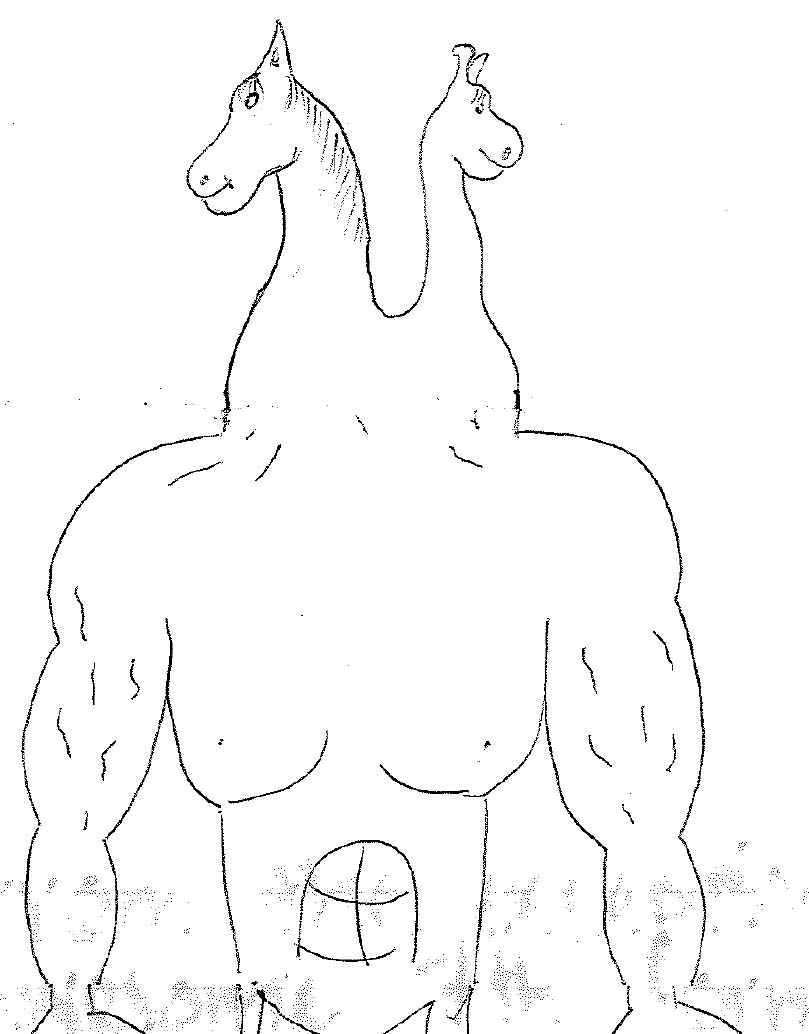
\includegraphics[height=3in]{images/bdaydrawingfromAlex.jpg}
	\caption{Drawing that Alex gave me the day after my birthday}
	\label{fig:bdaydrawing}
\end{figure}


\subsection{The Relaxed Group}
\isi{The Relaxed Group} was another group I came to know quite well. I was especially grateful for their presence on days when I was tired. I felt comfortable with them and accepted by them. Exchanges with them took less energy on my part. When I asked Megan and Anita if they would mind if I recorded them, they asked who I had already recorded. When I told them that I had already interviewed around 20 girls, they were shocked: Why wouldn't I ask them first?  They didn't seem as though their feelings were hurt; they simply seemed surprised that, given how close we were, they had not been among the first to be interviewed. Since graduation, I have met with Rose and Katrina and I am also still in contact with Megan.

\subsection{The Pasifika Group}
I became more and more familiar with \isi{The Pasifika Group} over time, especially with Marama. The girls in this group were especially interested in my California background: What was it like living near LA?  Are the boys better looking than here?  Have you ever met Snoop Dogg?  I enjoyed our conversations and it was my impression that they did, too. Although they were always friendly, I certainly never succeeded in feeling ``just like'' another girl in the group. They shared sensitive information with me, but they also adopted a more formal speaking register when addressing me directly. 

%At her friends' prompting, she showed me her latest design, a cute miniskirt that looked as though it could have been purchased from a shop.. , though they never invited me to join them outside of school grounds.

\subsection{The Goths}
\isi{The Goths} were very open with me from the beginning. They were talkative and they were quick to help shape my \isi{perception} of them. They invited me to join them during lunch or morning breaks and then would (in a friendly way) argue over who I would follow to class, explaining that I would learn more about life at SGH in one class over another. I felt as though I knew most of \isi{The Goths} very well.
 
\subsection{\isi{The Christians} and The Geeks} 
I am not Christian and I never once felt that Theresa and Esther needed me to be in order to interact with them or to be seen with them. In fact, they did not seem interested in whether or not I was Christian; they never asked and they always cheerfully accepted when I wanted to join them. Similarly, \isi{The Geeks} were always welcoming and I immediately felt accepted by them. 

\subsection{The Sporty Girls}
I came to know \isi{The Sporty Girls} early on. Though Naomi and Rachel were the first two I got to know, Kanani and I became the closest by the end of the year. I have met some of her family and we continue to stay in touch.

\subsection{Rochelle's Group}
I was very comfortable with Rochelle's Group and I believe they enjoyed my company as well. They asked me to come to parties and, of all the girls, they were the most persistent in insisting that I come to the formal. Part way through the year, they began to go to the school gym during lunch to work out instead of sitting in the CR or in their usual place on the lawn. I joined them in the gym on occasion, though I never had the proper clothes or shoes to join in on the workout. They continually invited me to parties and made sure that I never felt excluded from Year 13 events.

\subsection{Sonia's Group}
Of all of the groups presented here, I knew Sonia's group the least. I had the impression that they were not interested in me or what I was doing at the school. The phonetic analysis (Chapter \ref{ch:prod}) conducted on Holly's speech is based on a recording of a conversation between her and Sonia. I was in the room during the conversation, but I was not included in it. 

%   [maybe work this back in!!!! - already worked best bit in :) ]     With all of these different groups, I shifted my \isi{identity}. I felt compelled to behave in a way that they would like me, though there were boundaries. I did not join Emma (\isi{The PCs}), Megan (\isi{The Relaxed Group}), or Mariah (\isi{The Geeks}) in bad talking girls from other groups. My silence was often taken as ignorance of who the individual was, though there was an occasion where a racist comment from Onya prompted sidways glances at me from her friends and when met by silence (and a raised eyebrow) they told Onya not to say things like that. It was not always a conscious decision, but I was aware that I acted slightly differently with different groups.   Despite being one individual, my \isi{identity} was far from constant across the different groups. Does this affect my results?  And if so, how do I interpret them? 



\subsection{When research and friendship blend}

During the course of my work at SGH, there were several girls who were forced to deal with major life challenges such as eating disorders, pregnancy, miscarriage, and the death of parents and loved ones. To protect the individual girls, I will refrain from describing these in detail. Suffice it to say that the challenges faced by the girls of SGH were far from trivial and I found myself shifting between being a researcher and being a friend.

In conducting ethnography, the distinction between being a researcher and being a friend is sometimes blurred; in even a short amount of time, strong bonds can form \citep[79]{milroy1987}. Ethnographers become a part of the lives of the people they study, but some researchers may have qualms about getting too close to one's subjects: One does not want emotion to interfere with science. ``Without science, we lose our credibility. Without humanity, we lose our ability to understand others'' \citep[13]{agar1980}.

There were times when the girls tested the boundary between my roles as researcher and friend in places where I felt there should be one. For example, while walking to the supermarket one Study period with Renee, Alex, and Claudia (\isi{The Real Teenagers}), Alex commented that I could buy them alcohol, as none of them were yet 18. I could see her watching for my reaction and I treated it as a joke and laughed. That was not a boundary that I was willing to cross and, despite testing it, I do not believe that Alex expected that I would.

%And Onya invited me to Renee's birthday party. Given that several of the boys they were dating were roughly my age, I probably would not have 


There were other times when I dropped the \isi{identity} of researcher entirely and acted strictly as a friend, like the day that Sage collapsed. I had met Rose's sister, Sage, on a few different occasions, such as when she asked Rose to borrow lunch money. Sage was two years younger than Rose and seemed shy and sweet, but Rose worried about her. Sage's two best friends had decided that they would no longer be friends with her after ``borrowing'' a large sum of money. Soon thereafter, she was jumped and beaten up at a party. Then one day I witnessed something at the school and, embarrassingly, I did not respond as I should have. 

It was just before class began and I was talking with Maya (\isi{The BBs}) outside her classroom, which was one of many lined along the hall. Uniformed students stood in clumps talking, holding books and bags. A junior girl was pulling at her hair and I could see that she was trying to cover up a hickey. Out of the corner of my eye, I saw someone fall. I didn't see who it was and my view was obscured by three younger girls. I assumed it was someone messing around. Maya saw the fall, too, but kept talking, also assuming that it was some kind of joke. It wasn't. After what seemed like an eternity (but was probably more like ten seconds) I realised that the girl was not getting up. I pointed and asked if she was ok, at which point the girls blocking my view moved out of the way, though they kept staring at the girl on the floor. She was convulsing in what looked like an epileptic fit. I recognised her: It was Sage. A teacher saw her at the same time and rushed to her side. I told someone to get Rose. Someone else ran to fetch the school nurse. I stood waiting, watching Sage convulsing and wishing that I had acted sooner, wishing that I could do something. The bell rang and classes began, but there we were, separate from it all. Sage had stopped convulsing, but she remained on the floor. The teacher asked if she knew her name, if she knew the date. Sage did not answer and looked around blankly. 

\largerpage
When Rose arrived, she rushed to her sister's side. Rose talked to her softly and it looked as though Sage was answering. The nurse came in. She assured Rose that her sister would be fine and asked her to call their Mum. Rose and I went into a nearby classroom that was empty. She didn't want her sister to see her cry and didn't want her to know how worried she was. Rose called from my mobile phone, but her Mum didn't answer. Feeling scared and frustrated, she let her arms drop and threw her head back. I hugged her, assuring her that her sister would be fine. She cried and explained that her sister hadn't eaten and that the recent trauma combined with a lack of food may have caused her to faint. After several minutes, Rose began to calm down. She was able to reach her Mum and they went to the hospital for tests. 

I remained with Maya and the other girls in the hall, feeling vulnerable and helpless. I felt impressively insignificant. We were all in shock and felt uncertain of how to continue our day. I left school wondering what I could have done differently to help Sage sooner and wishing I had gone to the hospital with Rose. I wanted her to know that if she needed the support, I was there as a friend and not as the researcher who followed her and her friends around with a recorder. I texted her, asking how she was doing and asking whether Sage was ok. I got a text from Rose that night saying that Sage was fine and thanking me for helping. How had I helped?  I could have (and should have) done more, but all I did was give Rose a hug. 

I suspect that researchers in my field will come under fire if they get ``too close'' to the people they study because emotions could interfere with research-related judgments. But when faced with a crying girl who needs a friend, I will give her a hug if that's the best I can do at the time. Removing the human element from the methodology of ethnography is wrong and artificial.   How could I avoid being there for Rose as a friend?  And why would I want to avoid it?  She had shared her hardships and worries with me during the preceding months. Not only would it feel unnatural to dismiss our friendship on the basis of ``science'', it would be unethical.

%t's the human thing to do. I would go so far as to say that is unwilling to embrace the humanistic element of emotion in research is unfit to conduct this type of research. I genuinely liked the person she was. Furthermore, 

\subsection{Shaping interpretations}

How much were my interpretations of life at Selwyn Girls' High affected by my closeness with the girls, my own \isi{high school} experience, and my life prior to SGH in general?  Although I tried to go in open-minded, everyone's previous experiences inform the interpretations of new situations. \citet{mendozadenton2008} states explicitly that

\begin{quote}
	what I present as a text was filtered through my sensibility, my interpretation as well as my equivocation. Even what I noticed and considered as ``data points'' were selected in my \isi{perception} according to the sum of my prior experiences and my take on the situations encountered. \citep[44]{mendozadenton2008}
\end{quote}

\begin{quote}
	No ethnographer is a blank note\-pad just as no linguist is a tape re\-corder. \citep[48]{mendozadenton2008}
\end{quote}
 
\noindent It is the type of insight that would most easily be gleaned by an outsider who could view the entire situation (including me and my biases) from a different perspective. One effect of my personality that is obvious even to me is inherent in my interpretation of the incident with Rose's sister, Sage. The women in my family have a history of inheriting an irrational form of guilt from the women of the previous generation (which has the unfortunate effect of making the previous generation feel even more guilty). We take responsibility for the world's problems (e.g., children starving, greenhouse gases, the war in Iraq), not to mention problems in our personal lives, and feel guilty when we are unsuccessful in solving them. Sage's collapse was not my fault and many people would have responded the same way, yet I felt (and continue to feel) guilty that I did not do more to help. I recognise the lack of logic behind the guilt and I considered removing that aspect from the description of the incident from my dissertation and, later, this book. However, as it is, it is the honest portrayal of my interpretation of the situation. My inherited guilt combined with the close relationship that had developed between me and Rose served to shape how I viewed (and continue to view) what happened to her sister. I feel better acknowledging these effects and portraying my interpretation honestly rather than removing the emotions from the text. This way the reader can make up their own mind about how to interpret the situation without it being filtered through the reasoning of my self-conscious mind.

\begin{quote}
	On entering the community, an ethnographer carries more baggage than a tape recorder and a toothbrush, having grown up in a particular culture, acquiring many of its sometimes implicit assumptions about the nature of reality... The problem is not whether the ethnographer is biased; the problem is what kinds of biases exist - how do they enter into ethnographic work and how can their operation be documented. \citep[41-2]{agar1980}
\end{quote}

\noindent Interestingly, I also observed an influence in the opposite direction: I felt the memory of my own \isi{high school} life shift during my time at SGH. In the past, I had claimed that there were no cliques or ``popular girls'' where I went to \isi{high school}. After spending time at SGH, I realised that, like the CR girls, I had simply denied the reality of their existence. It took experiencing \isi{high school} life as an outsider for me to recognise and acknowledge this aspect of my own \isi{high school} life. This is not to say that my previous experiences did not help to shape my interpretations of the girls' socially constructed identities, but I was surprised to observe an effect in the opposite direction.

\section{Conclusion}

In sum, there were a number of groups at the school. The girls identified strongly with these groups and each girl found her own unique place within the group. Some of the groups (CR groups) valued conformity and viewed themselves as ``normal'' while other groups (\isi{NCR groups}) valued diversity and viewed themselves as different from the other girls. These aggregates of groups formed two distinct constellations of \isi{stance}. The following chapter investigates the degree to which phonetic variation at the school can be predicted by these different constellations. It also discusses the tendencies for particular girls to exhibit certain trends in the production of their speech and how these trends are consistent with non-linguistic expressions of their identities.


\newpage
\thispagestyle{empty}
\mbox{}